\documentclass[twoside]{book}

% Packages required by doxygen
\usepackage{fixltx2e}
\usepackage{calc}
\usepackage{doxygen}
\usepackage[export]{adjustbox} % also loads graphicx
\usepackage{graphicx}
\usepackage[utf8]{inputenc}
\usepackage{makeidx}
\usepackage{multicol}
\usepackage{multirow}
\PassOptionsToPackage{warn}{textcomp}
\usepackage{textcomp}
\usepackage[nointegrals]{wasysym}
\usepackage[table]{xcolor}

% Font selection
\usepackage[T1]{fontenc}
\usepackage[scaled=.90]{helvet}
\usepackage{courier}
\usepackage{amssymb}
\usepackage{sectsty}
\renewcommand{\familydefault}{\sfdefault}
\allsectionsfont{%
  \fontseries{bc}\selectfont%
  \color{darkgray}%
}
\renewcommand{\DoxyLabelFont}{%
  \fontseries{bc}\selectfont%
  \color{darkgray}%
}
\newcommand{\+}{\discretionary{\mbox{\scriptsize$\hookleftarrow$}}{}{}}

% Page & text layout
\usepackage{geometry}
\geometry{%
  a4paper,%
  top=2.5cm,%
  bottom=2.5cm,%
  left=2.5cm,%
  right=2.5cm%
}
\tolerance=750
\hfuzz=15pt
\hbadness=750
\setlength{\emergencystretch}{15pt}
\setlength{\parindent}{0cm}
\setlength{\parskip}{3ex plus 2ex minus 2ex}
\makeatletter
\renewcommand{\paragraph}{%
  \@startsection{paragraph}{4}{0ex}{-1.0ex}{1.0ex}{%
    \normalfont\normalsize\bfseries\SS@parafont%
  }%
}
\renewcommand{\subparagraph}{%
  \@startsection{subparagraph}{5}{0ex}{-1.0ex}{1.0ex}{%
    \normalfont\normalsize\bfseries\SS@subparafont%
  }%
}
\makeatother

% Headers & footers
\usepackage{fancyhdr}
\pagestyle{fancyplain}
\fancyhead[LE]{\fancyplain{}{\bfseries\thepage}}
\fancyhead[CE]{\fancyplain{}{}}
\fancyhead[RE]{\fancyplain{}{\bfseries\leftmark}}
\fancyhead[LO]{\fancyplain{}{\bfseries\rightmark}}
\fancyhead[CO]{\fancyplain{}{}}
\fancyhead[RO]{\fancyplain{}{\bfseries\thepage}}
\fancyfoot[LE]{\fancyplain{}{}}
\fancyfoot[CE]{\fancyplain{}{}}
\fancyfoot[RE]{\fancyplain{}{\bfseries\scriptsize Generated by Doxygen }}
\fancyfoot[LO]{\fancyplain{}{\bfseries\scriptsize Generated by Doxygen }}
\fancyfoot[CO]{\fancyplain{}{}}
\fancyfoot[RO]{\fancyplain{}{}}
\renewcommand{\footrulewidth}{0.4pt}
\renewcommand{\chaptermark}[1]{%
  \markboth{#1}{}%
}
\renewcommand{\sectionmark}[1]{%
  \markright{\thesection\ #1}%
}

% Indices & bibliography
\usepackage{natbib}
\usepackage[titles]{tocloft}
\setcounter{tocdepth}{3}
\setcounter{secnumdepth}{5}
\makeindex

% Hyperlinks (required, but should be loaded last)
\usepackage{ifpdf}
\ifpdf
  \usepackage[pdftex,pagebackref=true]{hyperref}
\else
  \usepackage[ps2pdf,pagebackref=true]{hyperref}
\fi
\hypersetup{%
  colorlinks=true,%
  linkcolor=blue,%
  citecolor=blue,%
  unicode%
}

% Custom commands
\newcommand{\clearemptydoublepage}{%
  \newpage{\pagestyle{empty}\cleardoublepage}%
}

\usepackage{caption}
\captionsetup{labelsep=space,justification=centering,font={bf},singlelinecheck=off,skip=4pt,position=top}

%===== C O N T E N T S =====

\begin{document}

% Titlepage & ToC
\hypersetup{pageanchor=false,
             bookmarksnumbered=true,
             pdfencoding=unicode
            }
\pagenumbering{alph}
\begin{titlepage}
\vspace*{7cm}
\begin{center}%
{\Large C\+Vector \\[1ex]\large 0.\+1.\+1 }\\
\vspace*{1cm}
{\large Generated by Doxygen 1.8.13}\\
\end{center}
\end{titlepage}
\clearemptydoublepage
\pagenumbering{roman}
\tableofcontents
\clearemptydoublepage
\pagenumbering{arabic}
\hypersetup{pageanchor=true}

%--- Begin generated contents ---
\chapter{Data Structure Index}
\section{Data Structures}
Here are the data structures with brief descriptions\+:\begin{DoxyCompactList}
\item\contentsline{section}{{\bf carray} }{\pageref{structcarray}}{}
\end{DoxyCompactList}

\chapter{File Index}
\section{File List}
Here is a list of all files with brief descriptions\+:\begin{DoxyCompactList}
\item\contentsline{section}{lib/\hyperlink{cvector__core_8h}{cvector\+\_\+core.\+h} }{\pageref{cvector__core_8h}}{}
\item\contentsline{section}{lib/\hyperlink{cvector__interface_8h}{cvector\+\_\+interface.\+h} }{\pageref{cvector__interface_8h}}{}
\end{DoxyCompactList}

\chapter{Data Structure Documentation}
\hypertarget{structcvector}{}\section{cvector Struct Reference}
\label{structcvector}\index{cvector@{cvector}}


{\ttfamily \#include $<$cvector\+\_\+interface.\+h$>$}

\subsection*{Data Fields}
\begin{DoxyCompactItemize}
\item 
\mbox{\Hypertarget{structcvector_a44c9984fcdd1c44d35235c67909dcc79}\label{structcvector_a44c9984fcdd1c44d35235c67909dcc79}} 
index\+\_\+t {\bfseries \+\_\+size}
\item 
\mbox{\Hypertarget{structcvector_a5948a8ef12921a8fc535fbcb48d4d4d4}\label{structcvector_a5948a8ef12921a8fc535fbcb48d4d4d4}} 
index\+\_\+t {\bfseries \+\_\+space}
\item 
\mbox{\Hypertarget{structcvector_ae60afc8a80c3a6c945520216265ebbe0}\label{structcvector_ae60afc8a80c3a6c945520216265ebbe0}} 
value\+\_\+t $\ast$ {\bfseries \+\_\+vector}
\end{DoxyCompactItemize}


\subsection{Detailed Description}
Main struct holding the cvector structure. 

Definition at line 190 of file cvector\+\_\+interface.\+h.



The documentation for this struct was generated from the following file\+:\begin{DoxyCompactItemize}
\item 
lib/cvector\+\_\+interface.\+h\end{DoxyCompactItemize}

\chapter{File Documentation}
\hypertarget{cvector_8h}{}\section{/home/thomas/\+Drive/tbagrel/dev/c/cvector/cvector.h File Reference}
\label{cvector_8h}\index{/home/thomas/\+Drive/tbagrel/dev/c/cvector/cvector.\+h@{/home/thomas/\+Drive/tbagrel/dev/c/cvector/cvector.\+h}}
{\ttfamily \#include $<$stdlib.\+h$>$}\newline
{\ttfamily \#include $<$stdint.\+h$>$}\newline
{\ttfamily \#include $<$inttypes.\+h$>$}\newline
{\ttfamily \#include $<$stdio.\+h$>$}\newline
{\ttfamily \#include $<$math.\+h$>$}\newline
{\ttfamily \#include $<$string.\+h$>$}\newline
{\ttfamily \#include $<$stdbool.\+h$>$}\newline
Include dependency graph for cvector.\+h\+:
\nopagebreak
\begin{figure}[H]
\begin{center}
\leavevmode
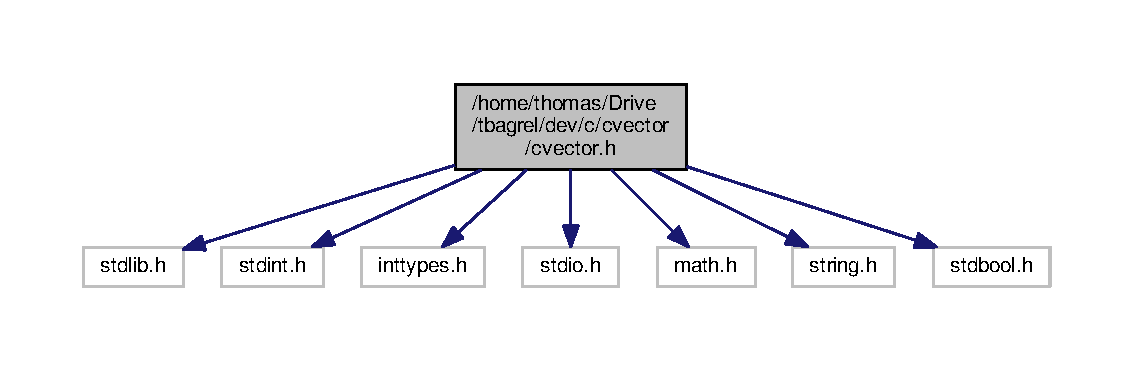
\includegraphics[width=350pt]{cvector_8h__incl}
\end{center}
\end{figure}
\subsection*{Data Structures}
\begin{DoxyCompactItemize}
\item 
struct \hyperlink{structcvector}{cvector}
\end{DoxyCompactItemize}
\subsection*{Macros}
\begin{DoxyCompactItemize}
\item 
\#define \hyperlink{cvector_8h_abd0abac859b89d3c63fd031ddf608a9e}{\+\_\+\+C\+O\+N\+C\+AT}(a,  b)~a \#\# b
\item 
\#define \hyperlink{cvector_8h_a88fa737059e67b4b17ec980e5877361e}{C\+O\+N\+C\+AT}(a,  b)~\hyperlink{cvector_8h_abd0abac859b89d3c63fd031ddf608a9e}{\+\_\+\+C\+O\+N\+C\+AT}(a, b)
\item 
\#define \hyperlink{cvector_8h_a29c765243a1c5b34627af48932ffc439}{D\+E\+F\+A\+U\+L\+T\+\_\+\+C\+V\+E\+C\+T\+O\+R\+\_\+T}~int
\item 
\#define \hyperlink{cvector_8h_acea3a56dc52185459f8966fece7b9671}{D\+E\+F\+A\+U\+L\+T\+\_\+\+D\+E\+F\+A\+U\+L\+T\+\_\+\+V\+A\+L\+UE}~0
\item 
\#define \hyperlink{cvector_8h_a816300364f1a38bd4c332a57792951f5}{D\+E\+F\+A\+U\+L\+T\+\_\+\+H\+A\+S\+H\+\_\+T}~size\+\_\+t
\item 
\#define \hyperlink{cvector_8h_af96f13eaf9d39f3aeb661fb99ca74409}{D\+E\+F\+A\+U\+L\+T\+\_\+\+P\+R\+I\+N\+T\+\_\+\+D\+E\+B\+U\+G\+\_\+\+F\+U\+NC}~\hyperlink{cvector_8h_ac2dbfacef236ca5daa1d3afb04c02724}{default\+\_\+print\+\_\+debug}
\item 
\#define \hyperlink{cvector_8h_ada843aff91b2ecd8122ae05adaed3db6}{P\+R\+I\+N\+T\+\_\+\+D\+E\+B\+UG}(level,  message)
\item 
\#define \hyperlink{cvector_8h_a18da678808a23365d00c58cdae11e29e}{D\+E\+F\+A\+U\+L\+T\+\_\+\+D\+E\+B\+U\+G\+\_\+\+L\+E\+V\+EL}~2
\item 
\#define \hyperlink{cvector_8h_a133390f76ff87262f4813b7948623a9c}{N\+O\+T\+\_\+\+F\+O\+U\+N\+D\+\_\+\+I\+N\+D\+EX}~((\hyperlink{cvector_8h_a05384666b24e4f096243ebf311436ee5}{index\+\_\+t}) (-\/1))
\item 
\#define \hyperlink{cvector_8h_ad24cec92ca2f0cfda6e9b53ea3dd1fc5}{R\+O\+U\+N\+D\+\_\+\+I\+N\+D\+EX}(x)~((\hyperlink{cvector_8h_a05384666b24e4f096243ebf311436ee5}{index\+\_\+t}) (lrint(x)))
\item 
\#define \hyperlink{cvector_8h_ac2d33ccaf63f5d5b66552b95426c0137}{D\+E\+B\+U\+G\+\_\+\+L\+E\+V\+EL}~\hyperlink{cvector_8h_a18da678808a23365d00c58cdae11e29e}{D\+E\+F\+A\+U\+L\+T\+\_\+\+D\+E\+B\+U\+G\+\_\+\+L\+E\+V\+EL}
\item 
\#define \hyperlink{cvector_8h_a3db9807a2d1fc2b1d0098e7ce8f7478b}{I\+N\+I\+T\+\_\+\+S\+P\+A\+CE}~8
\item 
\#define \hyperlink{cvector_8h_abf7442e3237b42ceb67324acea9a1d1c}{I\+N\+I\+T\+\_\+\+F\+A\+C\+T\+OR}~1.\+25
\item 
\#define \hyperlink{cvector_8h_abbdb13c8eb12c9460e8d0f39adfb88c8}{A\+D\+D\+S\+P\+A\+C\+E\+\_\+\+F\+A\+C\+T\+OR}~2.\+0
\item 
\#define \hyperlink{cvector_8h_a8e1a57dc5134ab73526871d11a622b68}{S\+H\+R\+I\+N\+K\+\_\+\+T\+H\+R\+E\+S\+H\+O\+LD}~0.\+5
\item 
\#define \hyperlink{cvector_8h_a31299318ba2f5406d7f7e2b299174e43}{S\+H\+R\+I\+N\+K\+\_\+\+F\+A\+C\+T\+OR}~0.\+5
\item 
\#define \hyperlink{cvector_8h_a77762dfca0730b89231a424d780ffa0a}{E\+X\+T\+E\+N\+D\+\_\+\+T\+H\+R\+E\+S\+H\+O\+LD}~0.\+90
\item 
\#define \hyperlink{cvector_8h_ac1443361a13d387b40da94941f0078dd}{E\+X\+T\+E\+N\+D\+\_\+\+F\+A\+C\+T\+OR}~2.\+0
\item 
\#define \hyperlink{cvector_8h_ae02a89ac32cbee34e2ef29f1e40ef58c}{P\+R\+I\+N\+T\+\_\+\+D\+E\+B\+U\+G\+\_\+\+F\+U\+NC}~\hyperlink{cvector_8h_af96f13eaf9d39f3aeb661fb99ca74409}{D\+E\+F\+A\+U\+L\+T\+\_\+\+P\+R\+I\+N\+T\+\_\+\+D\+E\+B\+U\+G\+\_\+\+F\+U\+NC}
\item 
\#define \hyperlink{cvector_8h_a5e15da722d5963a5f7bcef8bbbfa1638}{C\+V\+E\+C\+T\+O\+R\+\_\+T}~\hyperlink{cvector_8h_a29c765243a1c5b34627af48932ffc439}{D\+E\+F\+A\+U\+L\+T\+\_\+\+C\+V\+E\+C\+T\+O\+R\+\_\+T}
\item 
\#define \hyperlink{cvector_8h_a1683cf20cb6e91b381579ff93b309714}{D\+E\+F\+A\+U\+L\+T\+\_\+\+V\+A\+L\+UE}~\hyperlink{cvector_8h_acea3a56dc52185459f8966fece7b9671}{D\+E\+F\+A\+U\+L\+T\+\_\+\+D\+E\+F\+A\+U\+L\+T\+\_\+\+V\+A\+L\+UE}
\item 
\#define \hyperlink{cvector_8h_afe9a045b69b6db8ce1e1209cb3f23c80}{H\+A\+S\+H\+\_\+T}~\hyperlink{cvector_8h_a816300364f1a38bd4c332a57792951f5}{D\+E\+F\+A\+U\+L\+T\+\_\+\+H\+A\+S\+H\+\_\+T}
\item 
\#define \hyperlink{cvector_8h_a2d03a0c8fc8c754ba9895af080296662}{cvector}~\hyperlink{cvector_8h_a88fa737059e67b4b17ec980e5877361e}{C\+O\+N\+C\+AT}(\hyperlink{cvector_8h_a5e15da722d5963a5f7bcef8bbbfa1638}{C\+V\+E\+C\+T\+O\+R\+\_\+T}, \+\_\+cvector)
\item 
\#define \hyperlink{cvector_8h_af3643ddbd25169dad31b44b959394dc7}{cvector\+\_\+new}~\hyperlink{cvector_8h_a88fa737059e67b4b17ec980e5877361e}{C\+O\+N\+C\+AT}(\hyperlink{cvector_8h_a5e15da722d5963a5f7bcef8bbbfa1638}{C\+V\+E\+C\+T\+O\+R\+\_\+T}, \+\_\+cvector\+\_\+\+\_\+new)
\item 
\#define \hyperlink{cvector_8h_aca5164cb1aa88f7f19c4075d0bc5f805}{cvector\+\_\+new\+\_\+space}~\hyperlink{cvector_8h_a88fa737059e67b4b17ec980e5877361e}{C\+O\+N\+C\+AT}(\hyperlink{cvector_8h_a5e15da722d5963a5f7bcef8bbbfa1638}{C\+V\+E\+C\+T\+O\+R\+\_\+T}, \+\_\+cvector\+\_\+\+\_\+new\+\_\+space)
\item 
\#define \hyperlink{cvector_8h_abcbb5e5e4cdf38758949ca5f10c30e47}{cvector\+\_\+new\+\_\+copy}~\hyperlink{cvector_8h_a88fa737059e67b4b17ec980e5877361e}{C\+O\+N\+C\+AT}(\hyperlink{cvector_8h_a5e15da722d5963a5f7bcef8bbbfa1638}{C\+V\+E\+C\+T\+O\+R\+\_\+T}, \+\_\+cvector\+\_\+\+\_\+new\+\_\+copy)
\item 
\#define \hyperlink{cvector_8h_a0d8025e096c1aac2ebae9df97d78691d}{cvector\+\_\+new\+\_\+copy\+\_\+space}~\hyperlink{cvector_8h_a88fa737059e67b4b17ec980e5877361e}{C\+O\+N\+C\+AT}(\hyperlink{cvector_8h_a5e15da722d5963a5f7bcef8bbbfa1638}{C\+V\+E\+C\+T\+O\+R\+\_\+T}, \+\_\+cvector\+\_\+\+\_\+new\+\_\+copy\+\_\+space)
\item 
\#define \hyperlink{cvector_8h_a70f45a7f52f1338650da6361c6ed343f}{cvector\+\_\+free}~\hyperlink{cvector_8h_a88fa737059e67b4b17ec980e5877361e}{C\+O\+N\+C\+AT}(\hyperlink{cvector_8h_a5e15da722d5963a5f7bcef8bbbfa1638}{C\+V\+E\+C\+T\+O\+R\+\_\+T}, \+\_\+cvector\+\_\+\+\_\+free)
\item 
\#define \hyperlink{cvector_8h_af39d7cdb805176af722ef046a4a2b2c2}{cvector\+\_\+getsize}~\hyperlink{cvector_8h_a88fa737059e67b4b17ec980e5877361e}{C\+O\+N\+C\+AT}(\hyperlink{cvector_8h_a5e15da722d5963a5f7bcef8bbbfa1638}{C\+V\+E\+C\+T\+O\+R\+\_\+T}, \+\_\+cvector\+\_\+\+\_\+getsize)
\item 
\#define \hyperlink{cvector_8h_a373a516d422fd195c53c09c36cbe7d82}{cvector\+\_\+free\+\_\+func}~\hyperlink{cvector_8h_a88fa737059e67b4b17ec980e5877361e}{C\+O\+N\+C\+AT}(\hyperlink{cvector_8h_a5e15da722d5963a5f7bcef8bbbfa1638}{C\+V\+E\+C\+T\+O\+R\+\_\+T}, \+\_\+cvector\+\_\+\+\_\+free\+\_\+value)
\item 
\#define \hyperlink{cvector_8h_a9ed34c19cbe296317980c68d1797d146}{cvector\+\_\+add}~\hyperlink{cvector_8h_a88fa737059e67b4b17ec980e5877361e}{C\+O\+N\+C\+AT}(\hyperlink{cvector_8h_a5e15da722d5963a5f7bcef8bbbfa1638}{C\+V\+E\+C\+T\+O\+R\+\_\+T}, \+\_\+cvector\+\_\+\+\_\+add)
\item 
\#define \hyperlink{cvector_8h_a453850dca99e44eb36265c3bf3f9f73e}{cvector\+\_\+addi}~\hyperlink{cvector_8h_a88fa737059e67b4b17ec980e5877361e}{C\+O\+N\+C\+AT}(\hyperlink{cvector_8h_a5e15da722d5963a5f7bcef8bbbfa1638}{C\+V\+E\+C\+T\+O\+R\+\_\+T}, \+\_\+cvector\+\_\+\+\_\+addi)
\item 
\#define \hyperlink{cvector_8h_a43cb4f7b550a0b1a71e8b9d962806395}{cvector\+\_\+insert}~\hyperlink{cvector_8h_a88fa737059e67b4b17ec980e5877361e}{C\+O\+N\+C\+AT}(\hyperlink{cvector_8h_a5e15da722d5963a5f7bcef8bbbfa1638}{C\+V\+E\+C\+T\+O\+R\+\_\+T}, \+\_\+cvector\+\_\+\+\_\+insert)
\item 
\#define \hyperlink{cvector_8h_a07ebf34fb33362799534be60982d7cc8}{cvector\+\_\+remove}~\hyperlink{cvector_8h_a88fa737059e67b4b17ec980e5877361e}{C\+O\+N\+C\+AT}(\hyperlink{cvector_8h_a5e15da722d5963a5f7bcef8bbbfa1638}{C\+V\+E\+C\+T\+O\+R\+\_\+T}, \+\_\+cvector\+\_\+\+\_\+remove)
\item 
\#define \hyperlink{cvector_8h_a1424f999efb97f731ea07c85992b1259}{cvector\+\_\+removei}~\hyperlink{cvector_8h_a88fa737059e67b4b17ec980e5877361e}{C\+O\+N\+C\+AT}(\hyperlink{cvector_8h_a5e15da722d5963a5f7bcef8bbbfa1638}{C\+V\+E\+C\+T\+O\+R\+\_\+T}, \+\_\+cvector\+\_\+\+\_\+removei)
\item 
\#define \hyperlink{cvector_8h_a009303f26977e797d7c143e38c4d263e}{cvector\+\_\+drop}~\hyperlink{cvector_8h_a88fa737059e67b4b17ec980e5877361e}{C\+O\+N\+C\+AT}(\hyperlink{cvector_8h_a5e15da722d5963a5f7bcef8bbbfa1638}{C\+V\+E\+C\+T\+O\+R\+\_\+T}, \+\_\+cvector\+\_\+\+\_\+drop)
\item 
\#define \hyperlink{cvector_8h_a68ba6e77b57f0c0656f3d6e35c5d12da}{cvector\+\_\+clear}~\hyperlink{cvector_8h_a88fa737059e67b4b17ec980e5877361e}{C\+O\+N\+C\+AT}(\hyperlink{cvector_8h_a5e15da722d5963a5f7bcef8bbbfa1638}{C\+V\+E\+C\+T\+O\+R\+\_\+T}, \+\_\+cvector\+\_\+\+\_\+clear)
\item 
\#define \hyperlink{cvector_8h_a79baaa8927dfdf6635a321e277ae7f4e}{cvector\+\_\+get}~\hyperlink{cvector_8h_a88fa737059e67b4b17ec980e5877361e}{C\+O\+N\+C\+AT}(\hyperlink{cvector_8h_a5e15da722d5963a5f7bcef8bbbfa1638}{C\+V\+E\+C\+T\+O\+R\+\_\+T}, \+\_\+cvector\+\_\+\+\_\+get)
\item 
\#define \hyperlink{cvector_8h_a562157196361f6753556240eef4025de}{cvector\+\_\+safeget}~\hyperlink{cvector_8h_a88fa737059e67b4b17ec980e5877361e}{C\+O\+N\+C\+AT}(\hyperlink{cvector_8h_a5e15da722d5963a5f7bcef8bbbfa1638}{C\+V\+E\+C\+T\+O\+R\+\_\+T}, \+\_\+cvector\+\_\+\+\_\+safeget)
\item 
\#define \hyperlink{cvector_8h_a6ce1d1b0ccfe9af799dc66a8d4a86319}{cvector\+\_\+set}~\hyperlink{cvector_8h_a88fa737059e67b4b17ec980e5877361e}{C\+O\+N\+C\+AT}(\hyperlink{cvector_8h_a5e15da722d5963a5f7bcef8bbbfa1638}{C\+V\+E\+C\+T\+O\+R\+\_\+T}, \+\_\+cvector\+\_\+\+\_\+set)
\item 
\#define \hyperlink{cvector_8h_a3420c4176f753b105565826a15dcaf88}{cvector\+\_\+safeset}~\hyperlink{cvector_8h_a88fa737059e67b4b17ec980e5877361e}{C\+O\+N\+C\+AT}(\hyperlink{cvector_8h_a5e15da722d5963a5f7bcef8bbbfa1638}{C\+V\+E\+C\+T\+O\+R\+\_\+T}, \+\_\+cvector\+\_\+\+\_\+safeset)
\item 
\#define \hyperlink{cvector_8h_ae6531d1589b9362489cd95e86a985e93}{cvector\+\_\+appendto}~\hyperlink{cvector_8h_a88fa737059e67b4b17ec980e5877361e}{C\+O\+N\+C\+AT}(\hyperlink{cvector_8h_a5e15da722d5963a5f7bcef8bbbfa1638}{C\+V\+E\+C\+T\+O\+R\+\_\+T}, \+\_\+cvector\+\_\+\+\_\+appendto)
\item 
\#define \hyperlink{cvector_8h_abd428d4740573ce6e87dddb879589751}{cvector\+\_\+concat}~\hyperlink{cvector_8h_a88fa737059e67b4b17ec980e5877361e}{C\+O\+N\+C\+AT}(\hyperlink{cvector_8h_a5e15da722d5963a5f7bcef8bbbfa1638}{C\+V\+E\+C\+T\+O\+R\+\_\+T}, \+\_\+cvector\+\_\+\+\_\+concat)
\item 
\#define \hyperlink{cvector_8h_a5c16c9eb99c75ab12e1a2d3647ca8c21}{cvector\+\_\+reversed}~\hyperlink{cvector_8h_a88fa737059e67b4b17ec980e5877361e}{C\+O\+N\+C\+AT}(\hyperlink{cvector_8h_a5e15da722d5963a5f7bcef8bbbfa1638}{C\+V\+E\+C\+T\+O\+R\+\_\+T}, \+\_\+cvector\+\_\+\+\_\+reversed)
\item 
\#define \hyperlink{cvector_8h_a5ccf7fd8453004fb8e66572b60d8af73}{cvector\+\_\+hash}~\hyperlink{cvector_8h_a88fa737059e67b4b17ec980e5877361e}{C\+O\+N\+C\+AT}(\hyperlink{cvector_8h_a5e15da722d5963a5f7bcef8bbbfa1638}{C\+V\+E\+C\+T\+O\+R\+\_\+T}, \+\_\+cvector\+\_\+\+\_\+hash)
\item 
\#define \hyperlink{cvector_8h_ab07788ebb25a6870bde19ba5cbb61060}{cvector\+\_\+equal}~\hyperlink{cvector_8h_a88fa737059e67b4b17ec980e5877361e}{C\+O\+N\+C\+AT}(\hyperlink{cvector_8h_a5e15da722d5963a5f7bcef8bbbfa1638}{C\+V\+E\+C\+T\+O\+R\+\_\+T}, \+\_\+cvector\+\_\+\+\_\+equal)
\item 
\#define \hyperlink{cvector_8h_a17a4990f478c035ab4bef0716c7b9354}{cvector\+\_\+equal\+\_\+func}~\hyperlink{cvector_8h_a88fa737059e67b4b17ec980e5877361e}{C\+O\+N\+C\+AT}(\hyperlink{cvector_8h_a5e15da722d5963a5f7bcef8bbbfa1638}{C\+V\+E\+C\+T\+O\+R\+\_\+T}, \+\_\+cvector\+\_\+\+\_\+equal\+\_\+func)
\item 
\#define \hyperlink{cvector_8h_a385ae55033d32896e9d4be4325bea78c}{cvector\+\_\+toarray}~\hyperlink{cvector_8h_a88fa737059e67b4b17ec980e5877361e}{C\+O\+N\+C\+AT}(\hyperlink{cvector_8h_a5e15da722d5963a5f7bcef8bbbfa1638}{C\+V\+E\+C\+T\+O\+R\+\_\+T}, \+\_\+cvector\+\_\+\+\_\+toarray)
\item 
\#define \hyperlink{cvector_8h_ac937f9d34a8452ac8cc86687add5e24a}{cvector\+\_\+replace}~\hyperlink{cvector_8h_a88fa737059e67b4b17ec980e5877361e}{C\+O\+N\+C\+AT}(\hyperlink{cvector_8h_a5e15da722d5963a5f7bcef8bbbfa1638}{C\+V\+E\+C\+T\+O\+R\+\_\+T}, \+\_\+cvector\+\_\+\+\_\+replace)
\item 
\#define \hyperlink{cvector_8h_af9f756d04da4e4064d1934c4160c7f91}{cvector\+\_\+replace\+\_\+func}~\hyperlink{cvector_8h_a88fa737059e67b4b17ec980e5877361e}{C\+O\+N\+C\+AT}(\hyperlink{cvector_8h_a5e15da722d5963a5f7bcef8bbbfa1638}{C\+V\+E\+C\+T\+O\+R\+\_\+T}, \+\_\+cvector\+\_\+\+\_\+replace\+\_\+func)
\item 
\#define \hyperlink{cvector_8h_a1aa0dce34ea6ec1a2c066676cebf2a6a}{cvector\+\_\+sort}~\hyperlink{cvector_8h_a88fa737059e67b4b17ec980e5877361e}{C\+O\+N\+C\+AT}(\hyperlink{cvector_8h_a5e15da722d5963a5f7bcef8bbbfa1638}{C\+V\+E\+C\+T\+O\+R\+\_\+T}, \+\_\+cvector\+\_\+\+\_\+sort)
\item 
\#define \hyperlink{cvector_8h_a9757eab681e37499cd2c6b7d544162c9}{cvector\+\_\+indexof}~\hyperlink{cvector_8h_a88fa737059e67b4b17ec980e5877361e}{C\+O\+N\+C\+AT}(\hyperlink{cvector_8h_a5e15da722d5963a5f7bcef8bbbfa1638}{C\+V\+E\+C\+T\+O\+R\+\_\+T}, \+\_\+cvector\+\_\+\+\_\+indexof)
\item 
\#define \hyperlink{cvector_8h_a04d9b4e4e1e41eb48ce8114bd3f0912b}{cvector\+\_\+indexof\+\_\+func}~\hyperlink{cvector_8h_a88fa737059e67b4b17ec980e5877361e}{C\+O\+N\+C\+AT}(\hyperlink{cvector_8h_a5e15da722d5963a5f7bcef8bbbfa1638}{C\+V\+E\+C\+T\+O\+R\+\_\+T}, \+\_\+cvector\+\_\+\+\_\+indexof\+\_\+func)
\item 
\#define \hyperlink{cvector_8h_a4940acc3182042721bcf7102f2ceeb24}{cvector\+\_\+in}~\hyperlink{cvector_8h_a88fa737059e67b4b17ec980e5877361e}{C\+O\+N\+C\+AT}(\hyperlink{cvector_8h_a5e15da722d5963a5f7bcef8bbbfa1638}{C\+V\+E\+C\+T\+O\+R\+\_\+T}, \+\_\+cvector\+\_\+\+\_\+in)
\item 
\#define \hyperlink{cvector_8h_aa2b50973c47d37928b890217ca2eac2c}{cvector\+\_\+in\+\_\+func}~\hyperlink{cvector_8h_a88fa737059e67b4b17ec980e5877361e}{C\+O\+N\+C\+AT}(\hyperlink{cvector_8h_a5e15da722d5963a5f7bcef8bbbfa1638}{C\+V\+E\+C\+T\+O\+R\+\_\+T}, \+\_\+cvector\+\_\+\+\_\+in\+\_\+func)
\item 
\#define \hyperlink{cvector_8h_a19178a8e9548e20ef127fecc36df0bcf}{cvector\+\_\+slice}~\hyperlink{cvector_8h_a88fa737059e67b4b17ec980e5877361e}{C\+O\+N\+C\+AT}(\hyperlink{cvector_8h_a5e15da722d5963a5f7bcef8bbbfa1638}{C\+V\+E\+C\+T\+O\+R\+\_\+T}, \+\_\+cvector\+\_\+\+\_\+slice)
\item 
\#define \hyperlink{cvector_8h_aa222f3c71e732d2358f6cecb3bdda92f}{cvector\+\_\+slicetoarray}~\hyperlink{cvector_8h_a88fa737059e67b4b17ec980e5877361e}{C\+O\+N\+C\+AT}(\hyperlink{cvector_8h_a5e15da722d5963a5f7bcef8bbbfa1638}{C\+V\+E\+C\+T\+O\+R\+\_\+T}, \+\_\+cvector\+\_\+\+\_\+slicetoarray)
\item 
\#define \hyperlink{cvector_8h_a1aa368f3241a897fe78c3ffdbcbfca50}{cvector\+\_\+readjust}~\hyperlink{cvector_8h_a88fa737059e67b4b17ec980e5877361e}{C\+O\+N\+C\+AT}(\hyperlink{cvector_8h_a5e15da722d5963a5f7bcef8bbbfa1638}{C\+V\+E\+C\+T\+O\+R\+\_\+T}, \+\_\+cvector\+\_\+\+\_\+readjust)
\item 
\#define \hyperlink{cvector_8h_a4205916435bbfc3842cfd75a43e771ed}{cvector\+\_\+addspace}~\hyperlink{cvector_8h_a88fa737059e67b4b17ec980e5877361e}{C\+O\+N\+C\+AT}(\hyperlink{cvector_8h_a5e15da722d5963a5f7bcef8bbbfa1638}{C\+V\+E\+C\+T\+O\+R\+\_\+T}, \+\_\+cvector\+\_\+\+\_\+addspace)
\item 
\#define \hyperlink{cvector_8h_ad68f022487d0cc313c7ea50a183956c7}{\+\_\+\+\_\+cvector\+\_\+setspace}~\+\_\+\+\_\+\#\#\hyperlink{cvector_8h_a88fa737059e67b4b17ec980e5877361e}{C\+O\+N\+C\+AT}(\hyperlink{cvector_8h_a5e15da722d5963a5f7bcef8bbbfa1638}{C\+V\+E\+C\+T\+O\+R\+\_\+T}, \+\_\+cvector\+\_\+\+\_\+setspace)
\item 
\#define \hyperlink{cvector_8h_a14a1b75b7207d3da29cdca821c8c1545}{\+\_\+\+\_\+cvector\+\_\+shrink}~\+\_\+\+\_\+\#\#\hyperlink{cvector_8h_a88fa737059e67b4b17ec980e5877361e}{C\+O\+N\+C\+AT}(\hyperlink{cvector_8h_a5e15da722d5963a5f7bcef8bbbfa1638}{C\+V\+E\+C\+T\+O\+R\+\_\+T}, \+\_\+cvector\+\_\+\+\_\+shrink)
\item 
\#define \hyperlink{cvector_8h_a215ba71bba887f23a6b87fa73888b65d}{\+\_\+\+\_\+cvector\+\_\+extend}~\+\_\+\+\_\+\#\#\hyperlink{cvector_8h_a88fa737059e67b4b17ec980e5877361e}{C\+O\+N\+C\+AT}(\hyperlink{cvector_8h_a5e15da722d5963a5f7bcef8bbbfa1638}{C\+V\+E\+C\+T\+O\+R\+\_\+T}, \+\_\+cvector\+\_\+\+\_\+extend)
\end{DoxyCompactItemize}
\subsection*{Typedefs}
\begin{DoxyCompactItemize}
\item 
typedef size\+\_\+t \hyperlink{cvector_8h_a05384666b24e4f096243ebf311436ee5}{index\+\_\+t}
\item 
typedef \hyperlink{cvector_8h_a5e15da722d5963a5f7bcef8bbbfa1638}{C\+V\+E\+C\+T\+O\+R\+\_\+T} \hyperlink{cvector_8h_a02cdeb70a219711c52cec8d6d682048b}{value\+\_\+t}
\item 
typedef \hyperlink{cvector_8h_afe9a045b69b6db8ce1e1209cb3f23c80}{H\+A\+S\+H\+\_\+T} \hyperlink{cvector_8h_a814087d407b60e4d8b569f38370d30c9}{hash\+\_\+t}
\item 
typedef struct \hyperlink{structcvector}{cvector} \hyperlink{cvector_8h_ae8a3b37df7cac75e42faff09d0552627}{cvector}
\end{DoxyCompactItemize}
\subsection*{Functions}
\begin{DoxyCompactItemize}
\item 
void \hyperlink{cvector_8h_ac2dbfacef236ca5daa1d3afb04c02724}{default\+\_\+print\+\_\+debug} (int level, const char $\ast$message)
\item 
\hyperlink{structcvector}{cvector} $\ast$ \hyperlink{cvector_8h_a6442c91a2a3b14d4d1d865ba148c34e4}{cvector\+\_\+new} ()
\item 
\hyperlink{structcvector}{cvector} $\ast$ \hyperlink{cvector_8h_abc0d094d5cdbd31fc74f3902fd74a690}{cvector\+\_\+new\+\_\+space} (\hyperlink{cvector_8h_a05384666b24e4f096243ebf311436ee5}{index\+\_\+t} space)
\item 
\hyperlink{structcvector}{cvector} $\ast$ \hyperlink{cvector_8h_a5106edfcb490caa0a6eb53e4be088fa7}{cvector\+\_\+new\+\_\+copy} (\hyperlink{structcvector}{cvector} $\ast$p\+\_\+original)
\item 
\hyperlink{structcvector}{cvector} $\ast$ \hyperlink{cvector_8h_a8ae393983ad33cb1bc2df73f7d1db615}{cvector\+\_\+new\+\_\+copy\+\_\+space} (\hyperlink{structcvector}{cvector} $\ast$p\+\_\+original, \hyperlink{cvector_8h_a05384666b24e4f096243ebf311436ee5}{index\+\_\+t} space)
\item 
void \hyperlink{cvector_8h_a91b4f946caa0193dceb9afec7f54e7ff}{cvector\+\_\+free} (\hyperlink{structcvector}{cvector} $\ast$p\+\_\+cvector)
\item 
void \hyperlink{cvector_8h_a7ce27dde556f0de76df7c34a48e517a9}{cvector\+\_\+free\+\_\+func} (\hyperlink{structcvector}{cvector} $\ast$p\+\_\+vector, void($\ast$free\+\_\+value)(\hyperlink{cvector_8h_a02cdeb70a219711c52cec8d6d682048b}{value\+\_\+t}))
\item 
void \hyperlink{cvector_8h_ad504959e360214da1255d28534b1d3a4}{cvector\+\_\+add} (\hyperlink{structcvector}{cvector} $\ast$p\+\_\+cvector, \hyperlink{cvector_8h_a02cdeb70a219711c52cec8d6d682048b}{value\+\_\+t} value)
\item 
void \hyperlink{cvector_8h_aded13abbf232cf0d65c889cb806cee0b}{cvector\+\_\+addi} (\hyperlink{structcvector}{cvector} $\ast$p\+\_\+cvector, \hyperlink{cvector_8h_a02cdeb70a219711c52cec8d6d682048b}{value\+\_\+t} value, \hyperlink{cvector_8h_a05384666b24e4f096243ebf311436ee5}{index\+\_\+t} index)
\item 
\hyperlink{cvector_8h_a02cdeb70a219711c52cec8d6d682048b}{value\+\_\+t} \hyperlink{cvector_8h_a7af2a3f3b2e1fd3f2081536a4d73ac2e}{cvector\+\_\+remove} (\hyperlink{structcvector}{cvector} $\ast$p\+\_\+cvector)
\item 
\hyperlink{cvector_8h_a02cdeb70a219711c52cec8d6d682048b}{value\+\_\+t} \hyperlink{cvector_8h_aa10fda3704501241f975de8789dc5d9c}{cvector\+\_\+removei} (\hyperlink{structcvector}{cvector} $\ast$p\+\_\+cvector, \hyperlink{cvector_8h_a05384666b24e4f096243ebf311436ee5}{index\+\_\+t} index)
\item 
void \hyperlink{cvector_8h_aed9a4c7a1286857f5aa427938428b9f7}{cvector\+\_\+clear} (\hyperlink{structcvector}{cvector} $\ast$p\+\_\+cvector)
\item 
\hyperlink{cvector_8h_a02cdeb70a219711c52cec8d6d682048b}{value\+\_\+t} \hyperlink{cvector_8h_af9a92765b9a85699a7acba0c51ac8620}{cvector\+\_\+get} (\hyperlink{structcvector}{cvector} $\ast$p\+\_\+cvector, \hyperlink{cvector_8h_a05384666b24e4f096243ebf311436ee5}{index\+\_\+t} index)
\item 
\hyperlink{cvector_8h_a02cdeb70a219711c52cec8d6d682048b}{value\+\_\+t} \hyperlink{cvector_8h_a41b0ee17ac9cdc9967afb1dca8f9236a}{cvector\+\_\+safeget} (\hyperlink{structcvector}{cvector} $\ast$p\+\_\+cvector, \hyperlink{cvector_8h_a05384666b24e4f096243ebf311436ee5}{index\+\_\+t} index)
\item 
void \hyperlink{cvector_8h_a786ae2dbda0ab64599516679991eb93f}{cvector\+\_\+set} (\hyperlink{structcvector}{cvector} $\ast$p\+\_\+cvector, \hyperlink{cvector_8h_a02cdeb70a219711c52cec8d6d682048b}{value\+\_\+t} value, \hyperlink{cvector_8h_a05384666b24e4f096243ebf311436ee5}{index\+\_\+t} index)
\item 
void \hyperlink{cvector_8h_a2304a9cec856cf184ecaa057472fe2cf}{cvector\+\_\+safeset} (\hyperlink{structcvector}{cvector} $\ast$p\+\_\+cvector, \hyperlink{cvector_8h_a02cdeb70a219711c52cec8d6d682048b}{value\+\_\+t} value, \hyperlink{cvector_8h_a05384666b24e4f096243ebf311436ee5}{index\+\_\+t} index)
\item 
void \hyperlink{cvector_8h_ae23d89e171be11d31835926949af3de2}{cvector\+\_\+appendto} (\hyperlink{structcvector}{cvector} $\ast$p\+\_\+cvector, \hyperlink{structcvector}{cvector} $\ast$p\+\_\+add)
\item 
\hyperlink{structcvector}{cvector} $\ast$ \hyperlink{cvector_8h_a4a0181818d231d636c9de16a95efe931}{cvector\+\_\+concat} (\hyperlink{structcvector}{cvector} $\ast$p\+\_\+cvector\+\_\+1, \hyperlink{structcvector}{cvector} $\ast$p\+\_\+cvector\+\_\+2)
\item 
\hyperlink{structcvector}{cvector} $\ast$ \hyperlink{cvector_8h_af9185ec558ef030b082daee234f9312a}{cvector\+\_\+reversed} (\hyperlink{structcvector}{cvector} $\ast$p\+\_\+cvector)
\item 
\hyperlink{cvector_8h_a814087d407b60e4d8b569f38370d30c9}{hash\+\_\+t} \hyperlink{cvector_8h_ae5ad5e4e2a0c41c165d3ad1f933916e7}{cvector\+\_\+hash} (\hyperlink{structcvector}{cvector} $\ast$p\+\_\+cvector, \hyperlink{cvector_8h_a814087d407b60e4d8b569f38370d30c9}{hash\+\_\+t}($\ast$hash\+\_\+value)(\hyperlink{cvector_8h_a02cdeb70a219711c52cec8d6d682048b}{value\+\_\+t}))
\item 
bool \hyperlink{cvector_8h_aa0027f2467c3f04fb382dbec8cb6e33b}{cvector\+\_\+equal} (\hyperlink{structcvector}{cvector} $\ast$p\+\_\+cvector\+\_\+1, \hyperlink{structcvector}{cvector} $\ast$p\+\_\+cvector\+\_\+2)
\item 
bool \hyperlink{cvector_8h_aaf18bd41c613e955390bb26e6bf84ebb}{cvector\+\_\+equal\+\_\+func} (\hyperlink{structcvector}{cvector} $\ast$p\+\_\+cvector\+\_\+1, \hyperlink{structcvector}{cvector} $\ast$p\+\_\+cvector\+\_\+2, bool($\ast$equal\+\_\+value)(\hyperlink{cvector_8h_a02cdeb70a219711c52cec8d6d682048b}{value\+\_\+t}, \hyperlink{cvector_8h_a02cdeb70a219711c52cec8d6d682048b}{value\+\_\+t}))
\item 
\hyperlink{cvector_8h_a02cdeb70a219711c52cec8d6d682048b}{value\+\_\+t} $\ast$ \hyperlink{cvector_8h_acee2f57054d93a57da2b95f95df8fda8}{cvector\+\_\+toarray} (\hyperlink{structcvector}{cvector} $\ast$p\+\_\+cvector)
\item 
bool \hyperlink{cvector_8h_a3d72487e7685f7ab93fda40cabb60958}{cvector\+\_\+replace} (\hyperlink{structcvector}{cvector} $\ast$p\+\_\+cvector, \hyperlink{cvector_8h_a02cdeb70a219711c52cec8d6d682048b}{value\+\_\+t} original, \hyperlink{cvector_8h_a02cdeb70a219711c52cec8d6d682048b}{value\+\_\+t} replacement)
\item 
bool \hyperlink{cvector_8h_a8248626d0f31ebb5838c82d0a71f2b05}{cvector\+\_\+replace\+\_\+func} (\hyperlink{structcvector}{cvector} $\ast$p\+\_\+cvector, \hyperlink{cvector_8h_a02cdeb70a219711c52cec8d6d682048b}{value\+\_\+t} original, \hyperlink{cvector_8h_a02cdeb70a219711c52cec8d6d682048b}{value\+\_\+t} replacement, bool($\ast$equal\+\_\+value)(\hyperlink{cvector_8h_a02cdeb70a219711c52cec8d6d682048b}{value\+\_\+t}, \hyperlink{cvector_8h_a02cdeb70a219711c52cec8d6d682048b}{value\+\_\+t}))
\item 
void \hyperlink{cvector_8h_acf990e9a552f22bf18abfec4d2c14563}{cvector\+\_\+sort} (\hyperlink{structcvector}{cvector} $\ast$p\+\_\+cvector, int($\ast$comp\+\_\+value)(const void $\ast$, const void $\ast$))
\item 
\hyperlink{cvector_8h_a05384666b24e4f096243ebf311436ee5}{index\+\_\+t} \hyperlink{cvector_8h_aa11c7cb1423cfd6d9d41404188659f42}{cvector\+\_\+indexof} (\hyperlink{structcvector}{cvector} $\ast$p\+\_\+cvector, \hyperlink{cvector_8h_a02cdeb70a219711c52cec8d6d682048b}{value\+\_\+t} value)
\item 
\hyperlink{cvector_8h_a05384666b24e4f096243ebf311436ee5}{index\+\_\+t} \hyperlink{cvector_8h_a4d82b0c6d906d0b979ecabd6073ca242}{cvector\+\_\+indexof\+\_\+func} (\hyperlink{structcvector}{cvector} $\ast$p\+\_\+cvector, \hyperlink{cvector_8h_a02cdeb70a219711c52cec8d6d682048b}{value\+\_\+t} value, bool($\ast$equal\+\_\+value)(\hyperlink{cvector_8h_a02cdeb70a219711c52cec8d6d682048b}{value\+\_\+t}, \hyperlink{cvector_8h_a02cdeb70a219711c52cec8d6d682048b}{value\+\_\+t}))
\item 
\hyperlink{structcvector}{cvector} $\ast$ \hyperlink{cvector_8h_a58fc66f52658fce930c3fdd7116bf541}{cvector\+\_\+slice} (\hyperlink{structcvector}{cvector} $\ast$p\+\_\+cvector, \hyperlink{cvector_8h_a05384666b24e4f096243ebf311436ee5}{index\+\_\+t} from, \hyperlink{cvector_8h_a05384666b24e4f096243ebf311436ee5}{index\+\_\+t} to, \hyperlink{cvector_8h_a05384666b24e4f096243ebf311436ee5}{index\+\_\+t} step)
\item 
\hyperlink{cvector_8h_a02cdeb70a219711c52cec8d6d682048b}{value\+\_\+t} $\ast$ \hyperlink{cvector_8h_a06479149fcc3b358ac086aba792b19a7}{cvector\+\_\+slicetoarray} (\hyperlink{structcvector}{cvector} $\ast$p\+\_\+cvector, \hyperlink{cvector_8h_a05384666b24e4f096243ebf311436ee5}{index\+\_\+t} from, \hyperlink{cvector_8h_a05384666b24e4f096243ebf311436ee5}{index\+\_\+t} to, \hyperlink{cvector_8h_a05384666b24e4f096243ebf311436ee5}{index\+\_\+t} step)
\item 
void \hyperlink{cvector_8h_a9461750aa0be3a7104fca3ea80ea26e2}{cvector\+\_\+readjust} (\hyperlink{structcvector}{cvector} $\ast$p\+\_\+cvector)
\item 
void \hyperlink{cvector_8h_a2b3fb7098225f258606f6e87d51a293f}{\+\_\+\+\_\+cvector\+\_\+setspace} (\hyperlink{structcvector}{cvector} $\ast$p\+\_\+cvector, \hyperlink{cvector_8h_a05384666b24e4f096243ebf311436ee5}{index\+\_\+t} new\+\_\+space)
\end{DoxyCompactItemize}


\subsection{Macro Definition Documentation}
\mbox{\Hypertarget{cvector_8h_a215ba71bba887f23a6b87fa73888b65d}\label{cvector_8h_a215ba71bba887f23a6b87fa73888b65d}} 
\index{cvector.\+h@{cvector.\+h}!\+\_\+\+\_\+cvector\+\_\+extend@{\+\_\+\+\_\+cvector\+\_\+extend}}
\index{\+\_\+\+\_\+cvector\+\_\+extend@{\+\_\+\+\_\+cvector\+\_\+extend}!cvector.\+h@{cvector.\+h}}
\subsubsection{\texorpdfstring{\+\_\+\+\_\+cvector\+\_\+extend}{\_\_cvector\_extend}}
{\footnotesize\ttfamily \#define \+\_\+\+\_\+cvector\+\_\+extend~\+\_\+\+\_\+\#\#\hyperlink{cvector_8h_a88fa737059e67b4b17ec980e5877361e}{C\+O\+N\+C\+AT}(\hyperlink{cvector_8h_a5e15da722d5963a5f7bcef8bbbfa1638}{C\+V\+E\+C\+T\+O\+R\+\_\+T}, \+\_\+cvector\+\_\+\+\_\+extend)}



Definition at line 190 of file cvector.\+h.

\mbox{\Hypertarget{cvector_8h_ad68f022487d0cc313c7ea50a183956c7}\label{cvector_8h_ad68f022487d0cc313c7ea50a183956c7}} 
\index{cvector.\+h@{cvector.\+h}!\+\_\+\+\_\+cvector\+\_\+setspace@{\+\_\+\+\_\+cvector\+\_\+setspace}}
\index{\+\_\+\+\_\+cvector\+\_\+setspace@{\+\_\+\+\_\+cvector\+\_\+setspace}!cvector.\+h@{cvector.\+h}}
\subsubsection{\texorpdfstring{\+\_\+\+\_\+cvector\+\_\+setspace}{\_\_cvector\_setspace}}
{\footnotesize\ttfamily \#define \+\_\+\+\_\+cvector\+\_\+setspace~\+\_\+\+\_\+\#\#\hyperlink{cvector_8h_a88fa737059e67b4b17ec980e5877361e}{C\+O\+N\+C\+AT}(\hyperlink{cvector_8h_a5e15da722d5963a5f7bcef8bbbfa1638}{C\+V\+E\+C\+T\+O\+R\+\_\+T}, \+\_\+cvector\+\_\+\+\_\+setspace)}



Definition at line 188 of file cvector.\+h.

\mbox{\Hypertarget{cvector_8h_a14a1b75b7207d3da29cdca821c8c1545}\label{cvector_8h_a14a1b75b7207d3da29cdca821c8c1545}} 
\index{cvector.\+h@{cvector.\+h}!\+\_\+\+\_\+cvector\+\_\+shrink@{\+\_\+\+\_\+cvector\+\_\+shrink}}
\index{\+\_\+\+\_\+cvector\+\_\+shrink@{\+\_\+\+\_\+cvector\+\_\+shrink}!cvector.\+h@{cvector.\+h}}
\subsubsection{\texorpdfstring{\+\_\+\+\_\+cvector\+\_\+shrink}{\_\_cvector\_shrink}}
{\footnotesize\ttfamily \#define \+\_\+\+\_\+cvector\+\_\+shrink~\+\_\+\+\_\+\#\#\hyperlink{cvector_8h_a88fa737059e67b4b17ec980e5877361e}{C\+O\+N\+C\+AT}(\hyperlink{cvector_8h_a5e15da722d5963a5f7bcef8bbbfa1638}{C\+V\+E\+C\+T\+O\+R\+\_\+T}, \+\_\+cvector\+\_\+\+\_\+shrink)}



Definition at line 189 of file cvector.\+h.

\mbox{\Hypertarget{cvector_8h_abd0abac859b89d3c63fd031ddf608a9e}\label{cvector_8h_abd0abac859b89d3c63fd031ddf608a9e}} 
\index{cvector.\+h@{cvector.\+h}!\+\_\+\+C\+O\+N\+C\+AT@{\+\_\+\+C\+O\+N\+C\+AT}}
\index{\+\_\+\+C\+O\+N\+C\+AT@{\+\_\+\+C\+O\+N\+C\+AT}!cvector.\+h@{cvector.\+h}}
\subsubsection{\texorpdfstring{\+\_\+\+C\+O\+N\+C\+AT}{\_CONCAT}}
{\footnotesize\ttfamily \#define \+\_\+\+C\+O\+N\+C\+AT(\begin{DoxyParamCaption}\item[{}]{a,  }\item[{}]{b }\end{DoxyParamCaption})~a \#\# b}



Definition at line 13 of file cvector.\+h.

\mbox{\Hypertarget{cvector_8h_abbdb13c8eb12c9460e8d0f39adfb88c8}\label{cvector_8h_abbdb13c8eb12c9460e8d0f39adfb88c8}} 
\index{cvector.\+h@{cvector.\+h}!A\+D\+D\+S\+P\+A\+C\+E\+\_\+\+F\+A\+C\+T\+OR@{A\+D\+D\+S\+P\+A\+C\+E\+\_\+\+F\+A\+C\+T\+OR}}
\index{A\+D\+D\+S\+P\+A\+C\+E\+\_\+\+F\+A\+C\+T\+OR@{A\+D\+D\+S\+P\+A\+C\+E\+\_\+\+F\+A\+C\+T\+OR}!cvector.\+h@{cvector.\+h}}
\subsubsection{\texorpdfstring{A\+D\+D\+S\+P\+A\+C\+E\+\_\+\+F\+A\+C\+T\+OR}{ADDSPACE\_FACTOR}}
{\footnotesize\ttfamily \#define A\+D\+D\+S\+P\+A\+C\+E\+\_\+\+F\+A\+C\+T\+OR~2.\+0}

Space factor used when a cvector becomes too short to hold additional values. It means that the new cvector will have a space for A\+D\+D\+S\+P\+A\+C\+E\+\_\+\+F\+A\+C\+T\+OR
\begin{DoxyItemize}
\item the old space. 
\end{DoxyItemize}

Definition at line 73 of file cvector.\+h.

\mbox{\Hypertarget{cvector_8h_a88fa737059e67b4b17ec980e5877361e}\label{cvector_8h_a88fa737059e67b4b17ec980e5877361e}} 
\index{cvector.\+h@{cvector.\+h}!C\+O\+N\+C\+AT@{C\+O\+N\+C\+AT}}
\index{C\+O\+N\+C\+AT@{C\+O\+N\+C\+AT}!cvector.\+h@{cvector.\+h}}
\subsubsection{\texorpdfstring{C\+O\+N\+C\+AT}{CONCAT}}
{\footnotesize\ttfamily \#define C\+O\+N\+C\+AT(\begin{DoxyParamCaption}\item[{}]{a,  }\item[{}]{b }\end{DoxyParamCaption})~\hyperlink{cvector_8h_abd0abac859b89d3c63fd031ddf608a9e}{\+\_\+\+C\+O\+N\+C\+AT}(a, b)}



Definition at line 14 of file cvector.\+h.

\mbox{\Hypertarget{cvector_8h_a2d03a0c8fc8c754ba9895af080296662}\label{cvector_8h_a2d03a0c8fc8c754ba9895af080296662}} 
\index{cvector.\+h@{cvector.\+h}!cvector@{cvector}}
\index{cvector@{cvector}!cvector.\+h@{cvector.\+h}}
\subsubsection{\texorpdfstring{cvector}{cvector}}
{\footnotesize\ttfamily \#define \hyperlink{structcvector}{cvector}~\hyperlink{cvector_8h_a88fa737059e67b4b17ec980e5877361e}{C\+O\+N\+C\+AT}(\hyperlink{cvector_8h_a5e15da722d5963a5f7bcef8bbbfa1638}{C\+V\+E\+C\+T\+O\+R\+\_\+T}, \+\_\+cvector)}



Definition at line 151 of file cvector.\+h.

\mbox{\Hypertarget{cvector_8h_a9ed34c19cbe296317980c68d1797d146}\label{cvector_8h_a9ed34c19cbe296317980c68d1797d146}} 
\index{cvector.\+h@{cvector.\+h}!cvector\+\_\+add@{cvector\+\_\+add}}
\index{cvector\+\_\+add@{cvector\+\_\+add}!cvector.\+h@{cvector.\+h}}
\subsubsection{\texorpdfstring{cvector\+\_\+add}{cvector\_add}}
{\footnotesize\ttfamily \#define cvector\+\_\+add~\hyperlink{cvector_8h_a88fa737059e67b4b17ec980e5877361e}{C\+O\+N\+C\+AT}(\hyperlink{cvector_8h_a5e15da722d5963a5f7bcef8bbbfa1638}{C\+V\+E\+C\+T\+O\+R\+\_\+T}, \+\_\+cvector\+\_\+\+\_\+add)}



Definition at line 159 of file cvector.\+h.

\mbox{\Hypertarget{cvector_8h_a453850dca99e44eb36265c3bf3f9f73e}\label{cvector_8h_a453850dca99e44eb36265c3bf3f9f73e}} 
\index{cvector.\+h@{cvector.\+h}!cvector\+\_\+addi@{cvector\+\_\+addi}}
\index{cvector\+\_\+addi@{cvector\+\_\+addi}!cvector.\+h@{cvector.\+h}}
\subsubsection{\texorpdfstring{cvector\+\_\+addi}{cvector\_addi}}
{\footnotesize\ttfamily \#define cvector\+\_\+addi~\hyperlink{cvector_8h_a88fa737059e67b4b17ec980e5877361e}{C\+O\+N\+C\+AT}(\hyperlink{cvector_8h_a5e15da722d5963a5f7bcef8bbbfa1638}{C\+V\+E\+C\+T\+O\+R\+\_\+T}, \+\_\+cvector\+\_\+\+\_\+addi)}



Definition at line 160 of file cvector.\+h.

\mbox{\Hypertarget{cvector_8h_a4205916435bbfc3842cfd75a43e771ed}\label{cvector_8h_a4205916435bbfc3842cfd75a43e771ed}} 
\index{cvector.\+h@{cvector.\+h}!cvector\+\_\+addspace@{cvector\+\_\+addspace}}
\index{cvector\+\_\+addspace@{cvector\+\_\+addspace}!cvector.\+h@{cvector.\+h}}
\subsubsection{\texorpdfstring{cvector\+\_\+addspace}{cvector\_addspace}}
{\footnotesize\ttfamily \#define cvector\+\_\+addspace~\hyperlink{cvector_8h_a88fa737059e67b4b17ec980e5877361e}{C\+O\+N\+C\+AT}(\hyperlink{cvector_8h_a5e15da722d5963a5f7bcef8bbbfa1638}{C\+V\+E\+C\+T\+O\+R\+\_\+T}, \+\_\+cvector\+\_\+\+\_\+addspace)}



Definition at line 187 of file cvector.\+h.

\mbox{\Hypertarget{cvector_8h_ae6531d1589b9362489cd95e86a985e93}\label{cvector_8h_ae6531d1589b9362489cd95e86a985e93}} 
\index{cvector.\+h@{cvector.\+h}!cvector\+\_\+appendto@{cvector\+\_\+appendto}}
\index{cvector\+\_\+appendto@{cvector\+\_\+appendto}!cvector.\+h@{cvector.\+h}}
\subsubsection{\texorpdfstring{cvector\+\_\+appendto}{cvector\_appendto}}
{\footnotesize\ttfamily \#define cvector\+\_\+appendto~\hyperlink{cvector_8h_a88fa737059e67b4b17ec980e5877361e}{C\+O\+N\+C\+AT}(\hyperlink{cvector_8h_a5e15da722d5963a5f7bcef8bbbfa1638}{C\+V\+E\+C\+T\+O\+R\+\_\+T}, \+\_\+cvector\+\_\+\+\_\+appendto)}



Definition at line 170 of file cvector.\+h.

\mbox{\Hypertarget{cvector_8h_a68ba6e77b57f0c0656f3d6e35c5d12da}\label{cvector_8h_a68ba6e77b57f0c0656f3d6e35c5d12da}} 
\index{cvector.\+h@{cvector.\+h}!cvector\+\_\+clear@{cvector\+\_\+clear}}
\index{cvector\+\_\+clear@{cvector\+\_\+clear}!cvector.\+h@{cvector.\+h}}
\subsubsection{\texorpdfstring{cvector\+\_\+clear}{cvector\_clear}}
{\footnotesize\ttfamily \#define cvector\+\_\+clear~\hyperlink{cvector_8h_a88fa737059e67b4b17ec980e5877361e}{C\+O\+N\+C\+AT}(\hyperlink{cvector_8h_a5e15da722d5963a5f7bcef8bbbfa1638}{C\+V\+E\+C\+T\+O\+R\+\_\+T}, \+\_\+cvector\+\_\+\+\_\+clear)}



Definition at line 165 of file cvector.\+h.

\mbox{\Hypertarget{cvector_8h_abd428d4740573ce6e87dddb879589751}\label{cvector_8h_abd428d4740573ce6e87dddb879589751}} 
\index{cvector.\+h@{cvector.\+h}!cvector\+\_\+concat@{cvector\+\_\+concat}}
\index{cvector\+\_\+concat@{cvector\+\_\+concat}!cvector.\+h@{cvector.\+h}}
\subsubsection{\texorpdfstring{cvector\+\_\+concat}{cvector\_concat}}
{\footnotesize\ttfamily \#define cvector\+\_\+concat~\hyperlink{cvector_8h_a88fa737059e67b4b17ec980e5877361e}{C\+O\+N\+C\+AT}(\hyperlink{cvector_8h_a5e15da722d5963a5f7bcef8bbbfa1638}{C\+V\+E\+C\+T\+O\+R\+\_\+T}, \+\_\+cvector\+\_\+\+\_\+concat)}



Definition at line 171 of file cvector.\+h.

\mbox{\Hypertarget{cvector_8h_a009303f26977e797d7c143e38c4d263e}\label{cvector_8h_a009303f26977e797d7c143e38c4d263e}} 
\index{cvector.\+h@{cvector.\+h}!cvector\+\_\+drop@{cvector\+\_\+drop}}
\index{cvector\+\_\+drop@{cvector\+\_\+drop}!cvector.\+h@{cvector.\+h}}
\subsubsection{\texorpdfstring{cvector\+\_\+drop}{cvector\_drop}}
{\footnotesize\ttfamily \#define cvector\+\_\+drop~\hyperlink{cvector_8h_a88fa737059e67b4b17ec980e5877361e}{C\+O\+N\+C\+AT}(\hyperlink{cvector_8h_a5e15da722d5963a5f7bcef8bbbfa1638}{C\+V\+E\+C\+T\+O\+R\+\_\+T}, \+\_\+cvector\+\_\+\+\_\+drop)}



Definition at line 164 of file cvector.\+h.

\mbox{\Hypertarget{cvector_8h_ab07788ebb25a6870bde19ba5cbb61060}\label{cvector_8h_ab07788ebb25a6870bde19ba5cbb61060}} 
\index{cvector.\+h@{cvector.\+h}!cvector\+\_\+equal@{cvector\+\_\+equal}}
\index{cvector\+\_\+equal@{cvector\+\_\+equal}!cvector.\+h@{cvector.\+h}}
\subsubsection{\texorpdfstring{cvector\+\_\+equal}{cvector\_equal}}
{\footnotesize\ttfamily \#define cvector\+\_\+equal~\hyperlink{cvector_8h_a88fa737059e67b4b17ec980e5877361e}{C\+O\+N\+C\+AT}(\hyperlink{cvector_8h_a5e15da722d5963a5f7bcef8bbbfa1638}{C\+V\+E\+C\+T\+O\+R\+\_\+T}, \+\_\+cvector\+\_\+\+\_\+equal)}



Definition at line 174 of file cvector.\+h.

\mbox{\Hypertarget{cvector_8h_a17a4990f478c035ab4bef0716c7b9354}\label{cvector_8h_a17a4990f478c035ab4bef0716c7b9354}} 
\index{cvector.\+h@{cvector.\+h}!cvector\+\_\+equal\+\_\+func@{cvector\+\_\+equal\+\_\+func}}
\index{cvector\+\_\+equal\+\_\+func@{cvector\+\_\+equal\+\_\+func}!cvector.\+h@{cvector.\+h}}
\subsubsection{\texorpdfstring{cvector\+\_\+equal\+\_\+func}{cvector\_equal\_func}}
{\footnotesize\ttfamily \#define cvector\+\_\+equal\+\_\+func~\hyperlink{cvector_8h_a88fa737059e67b4b17ec980e5877361e}{C\+O\+N\+C\+AT}(\hyperlink{cvector_8h_a5e15da722d5963a5f7bcef8bbbfa1638}{C\+V\+E\+C\+T\+O\+R\+\_\+T}, \+\_\+cvector\+\_\+\+\_\+equal\+\_\+func)}



Definition at line 175 of file cvector.\+h.

\mbox{\Hypertarget{cvector_8h_a70f45a7f52f1338650da6361c6ed343f}\label{cvector_8h_a70f45a7f52f1338650da6361c6ed343f}} 
\index{cvector.\+h@{cvector.\+h}!cvector\+\_\+free@{cvector\+\_\+free}}
\index{cvector\+\_\+free@{cvector\+\_\+free}!cvector.\+h@{cvector.\+h}}
\subsubsection{\texorpdfstring{cvector\+\_\+free}{cvector\_free}}
{\footnotesize\ttfamily \#define cvector\+\_\+free~\hyperlink{cvector_8h_a88fa737059e67b4b17ec980e5877361e}{C\+O\+N\+C\+AT}(\hyperlink{cvector_8h_a5e15da722d5963a5f7bcef8bbbfa1638}{C\+V\+E\+C\+T\+O\+R\+\_\+T}, \+\_\+cvector\+\_\+\+\_\+free)}



Definition at line 156 of file cvector.\+h.

\mbox{\Hypertarget{cvector_8h_a373a516d422fd195c53c09c36cbe7d82}\label{cvector_8h_a373a516d422fd195c53c09c36cbe7d82}} 
\index{cvector.\+h@{cvector.\+h}!cvector\+\_\+free\+\_\+func@{cvector\+\_\+free\+\_\+func}}
\index{cvector\+\_\+free\+\_\+func@{cvector\+\_\+free\+\_\+func}!cvector.\+h@{cvector.\+h}}
\subsubsection{\texorpdfstring{cvector\+\_\+free\+\_\+func}{cvector\_free\_func}}
{\footnotesize\ttfamily \#define cvector\+\_\+free\+\_\+func~\hyperlink{cvector_8h_a88fa737059e67b4b17ec980e5877361e}{C\+O\+N\+C\+AT}(\hyperlink{cvector_8h_a5e15da722d5963a5f7bcef8bbbfa1638}{C\+V\+E\+C\+T\+O\+R\+\_\+T}, \+\_\+cvector\+\_\+\+\_\+free\+\_\+value)}



Definition at line 158 of file cvector.\+h.

\mbox{\Hypertarget{cvector_8h_a79baaa8927dfdf6635a321e277ae7f4e}\label{cvector_8h_a79baaa8927dfdf6635a321e277ae7f4e}} 
\index{cvector.\+h@{cvector.\+h}!cvector\+\_\+get@{cvector\+\_\+get}}
\index{cvector\+\_\+get@{cvector\+\_\+get}!cvector.\+h@{cvector.\+h}}
\subsubsection{\texorpdfstring{cvector\+\_\+get}{cvector\_get}}
{\footnotesize\ttfamily \#define cvector\+\_\+get~\hyperlink{cvector_8h_a88fa737059e67b4b17ec980e5877361e}{C\+O\+N\+C\+AT}(\hyperlink{cvector_8h_a5e15da722d5963a5f7bcef8bbbfa1638}{C\+V\+E\+C\+T\+O\+R\+\_\+T}, \+\_\+cvector\+\_\+\+\_\+get)}



Definition at line 166 of file cvector.\+h.

\mbox{\Hypertarget{cvector_8h_af39d7cdb805176af722ef046a4a2b2c2}\label{cvector_8h_af39d7cdb805176af722ef046a4a2b2c2}} 
\index{cvector.\+h@{cvector.\+h}!cvector\+\_\+getsize@{cvector\+\_\+getsize}}
\index{cvector\+\_\+getsize@{cvector\+\_\+getsize}!cvector.\+h@{cvector.\+h}}
\subsubsection{\texorpdfstring{cvector\+\_\+getsize}{cvector\_getsize}}
{\footnotesize\ttfamily \#define cvector\+\_\+getsize~\hyperlink{cvector_8h_a88fa737059e67b4b17ec980e5877361e}{C\+O\+N\+C\+AT}(\hyperlink{cvector_8h_a5e15da722d5963a5f7bcef8bbbfa1638}{C\+V\+E\+C\+T\+O\+R\+\_\+T}, \+\_\+cvector\+\_\+\+\_\+getsize)}



Definition at line 157 of file cvector.\+h.

\mbox{\Hypertarget{cvector_8h_a5ccf7fd8453004fb8e66572b60d8af73}\label{cvector_8h_a5ccf7fd8453004fb8e66572b60d8af73}} 
\index{cvector.\+h@{cvector.\+h}!cvector\+\_\+hash@{cvector\+\_\+hash}}
\index{cvector\+\_\+hash@{cvector\+\_\+hash}!cvector.\+h@{cvector.\+h}}
\subsubsection{\texorpdfstring{cvector\+\_\+hash}{cvector\_hash}}
{\footnotesize\ttfamily \#define cvector\+\_\+hash~\hyperlink{cvector_8h_a88fa737059e67b4b17ec980e5877361e}{C\+O\+N\+C\+AT}(\hyperlink{cvector_8h_a5e15da722d5963a5f7bcef8bbbfa1638}{C\+V\+E\+C\+T\+O\+R\+\_\+T}, \+\_\+cvector\+\_\+\+\_\+hash)}



Definition at line 173 of file cvector.\+h.

\mbox{\Hypertarget{cvector_8h_a4940acc3182042721bcf7102f2ceeb24}\label{cvector_8h_a4940acc3182042721bcf7102f2ceeb24}} 
\index{cvector.\+h@{cvector.\+h}!cvector\+\_\+in@{cvector\+\_\+in}}
\index{cvector\+\_\+in@{cvector\+\_\+in}!cvector.\+h@{cvector.\+h}}
\subsubsection{\texorpdfstring{cvector\+\_\+in}{cvector\_in}}
{\footnotesize\ttfamily \#define cvector\+\_\+in~\hyperlink{cvector_8h_a88fa737059e67b4b17ec980e5877361e}{C\+O\+N\+C\+AT}(\hyperlink{cvector_8h_a5e15da722d5963a5f7bcef8bbbfa1638}{C\+V\+E\+C\+T\+O\+R\+\_\+T}, \+\_\+cvector\+\_\+\+\_\+in)}



Definition at line 182 of file cvector.\+h.

\mbox{\Hypertarget{cvector_8h_aa2b50973c47d37928b890217ca2eac2c}\label{cvector_8h_aa2b50973c47d37928b890217ca2eac2c}} 
\index{cvector.\+h@{cvector.\+h}!cvector\+\_\+in\+\_\+func@{cvector\+\_\+in\+\_\+func}}
\index{cvector\+\_\+in\+\_\+func@{cvector\+\_\+in\+\_\+func}!cvector.\+h@{cvector.\+h}}
\subsubsection{\texorpdfstring{cvector\+\_\+in\+\_\+func}{cvector\_in\_func}}
{\footnotesize\ttfamily \#define cvector\+\_\+in\+\_\+func~\hyperlink{cvector_8h_a88fa737059e67b4b17ec980e5877361e}{C\+O\+N\+C\+AT}(\hyperlink{cvector_8h_a5e15da722d5963a5f7bcef8bbbfa1638}{C\+V\+E\+C\+T\+O\+R\+\_\+T}, \+\_\+cvector\+\_\+\+\_\+in\+\_\+func)}



Definition at line 183 of file cvector.\+h.

\mbox{\Hypertarget{cvector_8h_a9757eab681e37499cd2c6b7d544162c9}\label{cvector_8h_a9757eab681e37499cd2c6b7d544162c9}} 
\index{cvector.\+h@{cvector.\+h}!cvector\+\_\+indexof@{cvector\+\_\+indexof}}
\index{cvector\+\_\+indexof@{cvector\+\_\+indexof}!cvector.\+h@{cvector.\+h}}
\subsubsection{\texorpdfstring{cvector\+\_\+indexof}{cvector\_indexof}}
{\footnotesize\ttfamily \#define cvector\+\_\+indexof~\hyperlink{cvector_8h_a88fa737059e67b4b17ec980e5877361e}{C\+O\+N\+C\+AT}(\hyperlink{cvector_8h_a5e15da722d5963a5f7bcef8bbbfa1638}{C\+V\+E\+C\+T\+O\+R\+\_\+T}, \+\_\+cvector\+\_\+\+\_\+indexof)}



Definition at line 180 of file cvector.\+h.

\mbox{\Hypertarget{cvector_8h_a04d9b4e4e1e41eb48ce8114bd3f0912b}\label{cvector_8h_a04d9b4e4e1e41eb48ce8114bd3f0912b}} 
\index{cvector.\+h@{cvector.\+h}!cvector\+\_\+indexof\+\_\+func@{cvector\+\_\+indexof\+\_\+func}}
\index{cvector\+\_\+indexof\+\_\+func@{cvector\+\_\+indexof\+\_\+func}!cvector.\+h@{cvector.\+h}}
\subsubsection{\texorpdfstring{cvector\+\_\+indexof\+\_\+func}{cvector\_indexof\_func}}
{\footnotesize\ttfamily \#define cvector\+\_\+indexof\+\_\+func~\hyperlink{cvector_8h_a88fa737059e67b4b17ec980e5877361e}{C\+O\+N\+C\+AT}(\hyperlink{cvector_8h_a5e15da722d5963a5f7bcef8bbbfa1638}{C\+V\+E\+C\+T\+O\+R\+\_\+T}, \+\_\+cvector\+\_\+\+\_\+indexof\+\_\+func)}



Definition at line 181 of file cvector.\+h.

\mbox{\Hypertarget{cvector_8h_a43cb4f7b550a0b1a71e8b9d962806395}\label{cvector_8h_a43cb4f7b550a0b1a71e8b9d962806395}} 
\index{cvector.\+h@{cvector.\+h}!cvector\+\_\+insert@{cvector\+\_\+insert}}
\index{cvector\+\_\+insert@{cvector\+\_\+insert}!cvector.\+h@{cvector.\+h}}
\subsubsection{\texorpdfstring{cvector\+\_\+insert}{cvector\_insert}}
{\footnotesize\ttfamily \#define cvector\+\_\+insert~\hyperlink{cvector_8h_a88fa737059e67b4b17ec980e5877361e}{C\+O\+N\+C\+AT}(\hyperlink{cvector_8h_a5e15da722d5963a5f7bcef8bbbfa1638}{C\+V\+E\+C\+T\+O\+R\+\_\+T}, \+\_\+cvector\+\_\+\+\_\+insert)}



Definition at line 161 of file cvector.\+h.

\mbox{\Hypertarget{cvector_8h_af3643ddbd25169dad31b44b959394dc7}\label{cvector_8h_af3643ddbd25169dad31b44b959394dc7}} 
\index{cvector.\+h@{cvector.\+h}!cvector\+\_\+new@{cvector\+\_\+new}}
\index{cvector\+\_\+new@{cvector\+\_\+new}!cvector.\+h@{cvector.\+h}}
\subsubsection{\texorpdfstring{cvector\+\_\+new}{cvector\_new}}
{\footnotesize\ttfamily \#define cvector\+\_\+new~\hyperlink{cvector_8h_a88fa737059e67b4b17ec980e5877361e}{C\+O\+N\+C\+AT}(\hyperlink{cvector_8h_a5e15da722d5963a5f7bcef8bbbfa1638}{C\+V\+E\+C\+T\+O\+R\+\_\+T}, \+\_\+cvector\+\_\+\+\_\+new)}



Definition at line 152 of file cvector.\+h.

\mbox{\Hypertarget{cvector_8h_abcbb5e5e4cdf38758949ca5f10c30e47}\label{cvector_8h_abcbb5e5e4cdf38758949ca5f10c30e47}} 
\index{cvector.\+h@{cvector.\+h}!cvector\+\_\+new\+\_\+copy@{cvector\+\_\+new\+\_\+copy}}
\index{cvector\+\_\+new\+\_\+copy@{cvector\+\_\+new\+\_\+copy}!cvector.\+h@{cvector.\+h}}
\subsubsection{\texorpdfstring{cvector\+\_\+new\+\_\+copy}{cvector\_new\_copy}}
{\footnotesize\ttfamily \#define cvector\+\_\+new\+\_\+copy~\hyperlink{cvector_8h_a88fa737059e67b4b17ec980e5877361e}{C\+O\+N\+C\+AT}(\hyperlink{cvector_8h_a5e15da722d5963a5f7bcef8bbbfa1638}{C\+V\+E\+C\+T\+O\+R\+\_\+T}, \+\_\+cvector\+\_\+\+\_\+new\+\_\+copy)}



Definition at line 154 of file cvector.\+h.

\mbox{\Hypertarget{cvector_8h_a0d8025e096c1aac2ebae9df97d78691d}\label{cvector_8h_a0d8025e096c1aac2ebae9df97d78691d}} 
\index{cvector.\+h@{cvector.\+h}!cvector\+\_\+new\+\_\+copy\+\_\+space@{cvector\+\_\+new\+\_\+copy\+\_\+space}}
\index{cvector\+\_\+new\+\_\+copy\+\_\+space@{cvector\+\_\+new\+\_\+copy\+\_\+space}!cvector.\+h@{cvector.\+h}}
\subsubsection{\texorpdfstring{cvector\+\_\+new\+\_\+copy\+\_\+space}{cvector\_new\_copy\_space}}
{\footnotesize\ttfamily \#define cvector\+\_\+new\+\_\+copy\+\_\+space~\hyperlink{cvector_8h_a88fa737059e67b4b17ec980e5877361e}{C\+O\+N\+C\+AT}(\hyperlink{cvector_8h_a5e15da722d5963a5f7bcef8bbbfa1638}{C\+V\+E\+C\+T\+O\+R\+\_\+T}, \+\_\+cvector\+\_\+\+\_\+new\+\_\+copy\+\_\+space)}



Definition at line 155 of file cvector.\+h.

\mbox{\Hypertarget{cvector_8h_aca5164cb1aa88f7f19c4075d0bc5f805}\label{cvector_8h_aca5164cb1aa88f7f19c4075d0bc5f805}} 
\index{cvector.\+h@{cvector.\+h}!cvector\+\_\+new\+\_\+space@{cvector\+\_\+new\+\_\+space}}
\index{cvector\+\_\+new\+\_\+space@{cvector\+\_\+new\+\_\+space}!cvector.\+h@{cvector.\+h}}
\subsubsection{\texorpdfstring{cvector\+\_\+new\+\_\+space}{cvector\_new\_space}}
{\footnotesize\ttfamily \#define cvector\+\_\+new\+\_\+space~\hyperlink{cvector_8h_a88fa737059e67b4b17ec980e5877361e}{C\+O\+N\+C\+AT}(\hyperlink{cvector_8h_a5e15da722d5963a5f7bcef8bbbfa1638}{C\+V\+E\+C\+T\+O\+R\+\_\+T}, \+\_\+cvector\+\_\+\+\_\+new\+\_\+space)}



Definition at line 153 of file cvector.\+h.

\mbox{\Hypertarget{cvector_8h_a1aa368f3241a897fe78c3ffdbcbfca50}\label{cvector_8h_a1aa368f3241a897fe78c3ffdbcbfca50}} 
\index{cvector.\+h@{cvector.\+h}!cvector\+\_\+readjust@{cvector\+\_\+readjust}}
\index{cvector\+\_\+readjust@{cvector\+\_\+readjust}!cvector.\+h@{cvector.\+h}}
\subsubsection{\texorpdfstring{cvector\+\_\+readjust}{cvector\_readjust}}
{\footnotesize\ttfamily \#define cvector\+\_\+readjust~\hyperlink{cvector_8h_a88fa737059e67b4b17ec980e5877361e}{C\+O\+N\+C\+AT}(\hyperlink{cvector_8h_a5e15da722d5963a5f7bcef8bbbfa1638}{C\+V\+E\+C\+T\+O\+R\+\_\+T}, \+\_\+cvector\+\_\+\+\_\+readjust)}



Definition at line 186 of file cvector.\+h.

\mbox{\Hypertarget{cvector_8h_a07ebf34fb33362799534be60982d7cc8}\label{cvector_8h_a07ebf34fb33362799534be60982d7cc8}} 
\index{cvector.\+h@{cvector.\+h}!cvector\+\_\+remove@{cvector\+\_\+remove}}
\index{cvector\+\_\+remove@{cvector\+\_\+remove}!cvector.\+h@{cvector.\+h}}
\subsubsection{\texorpdfstring{cvector\+\_\+remove}{cvector\_remove}}
{\footnotesize\ttfamily \#define cvector\+\_\+remove~\hyperlink{cvector_8h_a88fa737059e67b4b17ec980e5877361e}{C\+O\+N\+C\+AT}(\hyperlink{cvector_8h_a5e15da722d5963a5f7bcef8bbbfa1638}{C\+V\+E\+C\+T\+O\+R\+\_\+T}, \+\_\+cvector\+\_\+\+\_\+remove)}



Definition at line 162 of file cvector.\+h.

\mbox{\Hypertarget{cvector_8h_a1424f999efb97f731ea07c85992b1259}\label{cvector_8h_a1424f999efb97f731ea07c85992b1259}} 
\index{cvector.\+h@{cvector.\+h}!cvector\+\_\+removei@{cvector\+\_\+removei}}
\index{cvector\+\_\+removei@{cvector\+\_\+removei}!cvector.\+h@{cvector.\+h}}
\subsubsection{\texorpdfstring{cvector\+\_\+removei}{cvector\_removei}}
{\footnotesize\ttfamily \#define cvector\+\_\+removei~\hyperlink{cvector_8h_a88fa737059e67b4b17ec980e5877361e}{C\+O\+N\+C\+AT}(\hyperlink{cvector_8h_a5e15da722d5963a5f7bcef8bbbfa1638}{C\+V\+E\+C\+T\+O\+R\+\_\+T}, \+\_\+cvector\+\_\+\+\_\+removei)}



Definition at line 163 of file cvector.\+h.

\mbox{\Hypertarget{cvector_8h_ac937f9d34a8452ac8cc86687add5e24a}\label{cvector_8h_ac937f9d34a8452ac8cc86687add5e24a}} 
\index{cvector.\+h@{cvector.\+h}!cvector\+\_\+replace@{cvector\+\_\+replace}}
\index{cvector\+\_\+replace@{cvector\+\_\+replace}!cvector.\+h@{cvector.\+h}}
\subsubsection{\texorpdfstring{cvector\+\_\+replace}{cvector\_replace}}
{\footnotesize\ttfamily \#define cvector\+\_\+replace~\hyperlink{cvector_8h_a88fa737059e67b4b17ec980e5877361e}{C\+O\+N\+C\+AT}(\hyperlink{cvector_8h_a5e15da722d5963a5f7bcef8bbbfa1638}{C\+V\+E\+C\+T\+O\+R\+\_\+T}, \+\_\+cvector\+\_\+\+\_\+replace)}



Definition at line 177 of file cvector.\+h.

\mbox{\Hypertarget{cvector_8h_af9f756d04da4e4064d1934c4160c7f91}\label{cvector_8h_af9f756d04da4e4064d1934c4160c7f91}} 
\index{cvector.\+h@{cvector.\+h}!cvector\+\_\+replace\+\_\+func@{cvector\+\_\+replace\+\_\+func}}
\index{cvector\+\_\+replace\+\_\+func@{cvector\+\_\+replace\+\_\+func}!cvector.\+h@{cvector.\+h}}
\subsubsection{\texorpdfstring{cvector\+\_\+replace\+\_\+func}{cvector\_replace\_func}}
{\footnotesize\ttfamily \#define cvector\+\_\+replace\+\_\+func~\hyperlink{cvector_8h_a88fa737059e67b4b17ec980e5877361e}{C\+O\+N\+C\+AT}(\hyperlink{cvector_8h_a5e15da722d5963a5f7bcef8bbbfa1638}{C\+V\+E\+C\+T\+O\+R\+\_\+T}, \+\_\+cvector\+\_\+\+\_\+replace\+\_\+func)}



Definition at line 178 of file cvector.\+h.

\mbox{\Hypertarget{cvector_8h_a5c16c9eb99c75ab12e1a2d3647ca8c21}\label{cvector_8h_a5c16c9eb99c75ab12e1a2d3647ca8c21}} 
\index{cvector.\+h@{cvector.\+h}!cvector\+\_\+reversed@{cvector\+\_\+reversed}}
\index{cvector\+\_\+reversed@{cvector\+\_\+reversed}!cvector.\+h@{cvector.\+h}}
\subsubsection{\texorpdfstring{cvector\+\_\+reversed}{cvector\_reversed}}
{\footnotesize\ttfamily \#define cvector\+\_\+reversed~\hyperlink{cvector_8h_a88fa737059e67b4b17ec980e5877361e}{C\+O\+N\+C\+AT}(\hyperlink{cvector_8h_a5e15da722d5963a5f7bcef8bbbfa1638}{C\+V\+E\+C\+T\+O\+R\+\_\+T}, \+\_\+cvector\+\_\+\+\_\+reversed)}



Definition at line 172 of file cvector.\+h.

\mbox{\Hypertarget{cvector_8h_a562157196361f6753556240eef4025de}\label{cvector_8h_a562157196361f6753556240eef4025de}} 
\index{cvector.\+h@{cvector.\+h}!cvector\+\_\+safeget@{cvector\+\_\+safeget}}
\index{cvector\+\_\+safeget@{cvector\+\_\+safeget}!cvector.\+h@{cvector.\+h}}
\subsubsection{\texorpdfstring{cvector\+\_\+safeget}{cvector\_safeget}}
{\footnotesize\ttfamily \#define cvector\+\_\+safeget~\hyperlink{cvector_8h_a88fa737059e67b4b17ec980e5877361e}{C\+O\+N\+C\+AT}(\hyperlink{cvector_8h_a5e15da722d5963a5f7bcef8bbbfa1638}{C\+V\+E\+C\+T\+O\+R\+\_\+T}, \+\_\+cvector\+\_\+\+\_\+safeget)}



Definition at line 167 of file cvector.\+h.

\mbox{\Hypertarget{cvector_8h_a3420c4176f753b105565826a15dcaf88}\label{cvector_8h_a3420c4176f753b105565826a15dcaf88}} 
\index{cvector.\+h@{cvector.\+h}!cvector\+\_\+safeset@{cvector\+\_\+safeset}}
\index{cvector\+\_\+safeset@{cvector\+\_\+safeset}!cvector.\+h@{cvector.\+h}}
\subsubsection{\texorpdfstring{cvector\+\_\+safeset}{cvector\_safeset}}
{\footnotesize\ttfamily \#define cvector\+\_\+safeset~\hyperlink{cvector_8h_a88fa737059e67b4b17ec980e5877361e}{C\+O\+N\+C\+AT}(\hyperlink{cvector_8h_a5e15da722d5963a5f7bcef8bbbfa1638}{C\+V\+E\+C\+T\+O\+R\+\_\+T}, \+\_\+cvector\+\_\+\+\_\+safeset)}



Definition at line 169 of file cvector.\+h.

\mbox{\Hypertarget{cvector_8h_a6ce1d1b0ccfe9af799dc66a8d4a86319}\label{cvector_8h_a6ce1d1b0ccfe9af799dc66a8d4a86319}} 
\index{cvector.\+h@{cvector.\+h}!cvector\+\_\+set@{cvector\+\_\+set}}
\index{cvector\+\_\+set@{cvector\+\_\+set}!cvector.\+h@{cvector.\+h}}
\subsubsection{\texorpdfstring{cvector\+\_\+set}{cvector\_set}}
{\footnotesize\ttfamily \#define cvector\+\_\+set~\hyperlink{cvector_8h_a88fa737059e67b4b17ec980e5877361e}{C\+O\+N\+C\+AT}(\hyperlink{cvector_8h_a5e15da722d5963a5f7bcef8bbbfa1638}{C\+V\+E\+C\+T\+O\+R\+\_\+T}, \+\_\+cvector\+\_\+\+\_\+set)}



Definition at line 168 of file cvector.\+h.

\mbox{\Hypertarget{cvector_8h_a19178a8e9548e20ef127fecc36df0bcf}\label{cvector_8h_a19178a8e9548e20ef127fecc36df0bcf}} 
\index{cvector.\+h@{cvector.\+h}!cvector\+\_\+slice@{cvector\+\_\+slice}}
\index{cvector\+\_\+slice@{cvector\+\_\+slice}!cvector.\+h@{cvector.\+h}}
\subsubsection{\texorpdfstring{cvector\+\_\+slice}{cvector\_slice}}
{\footnotesize\ttfamily \#define cvector\+\_\+slice~\hyperlink{cvector_8h_a88fa737059e67b4b17ec980e5877361e}{C\+O\+N\+C\+AT}(\hyperlink{cvector_8h_a5e15da722d5963a5f7bcef8bbbfa1638}{C\+V\+E\+C\+T\+O\+R\+\_\+T}, \+\_\+cvector\+\_\+\+\_\+slice)}



Definition at line 184 of file cvector.\+h.

\mbox{\Hypertarget{cvector_8h_aa222f3c71e732d2358f6cecb3bdda92f}\label{cvector_8h_aa222f3c71e732d2358f6cecb3bdda92f}} 
\index{cvector.\+h@{cvector.\+h}!cvector\+\_\+slicetoarray@{cvector\+\_\+slicetoarray}}
\index{cvector\+\_\+slicetoarray@{cvector\+\_\+slicetoarray}!cvector.\+h@{cvector.\+h}}
\subsubsection{\texorpdfstring{cvector\+\_\+slicetoarray}{cvector\_slicetoarray}}
{\footnotesize\ttfamily \#define cvector\+\_\+slicetoarray~\hyperlink{cvector_8h_a88fa737059e67b4b17ec980e5877361e}{C\+O\+N\+C\+AT}(\hyperlink{cvector_8h_a5e15da722d5963a5f7bcef8bbbfa1638}{C\+V\+E\+C\+T\+O\+R\+\_\+T}, \+\_\+cvector\+\_\+\+\_\+slicetoarray)}



Definition at line 185 of file cvector.\+h.

\mbox{\Hypertarget{cvector_8h_a1aa0dce34ea6ec1a2c066676cebf2a6a}\label{cvector_8h_a1aa0dce34ea6ec1a2c066676cebf2a6a}} 
\index{cvector.\+h@{cvector.\+h}!cvector\+\_\+sort@{cvector\+\_\+sort}}
\index{cvector\+\_\+sort@{cvector\+\_\+sort}!cvector.\+h@{cvector.\+h}}
\subsubsection{\texorpdfstring{cvector\+\_\+sort}{cvector\_sort}}
{\footnotesize\ttfamily \#define cvector\+\_\+sort~\hyperlink{cvector_8h_a88fa737059e67b4b17ec980e5877361e}{C\+O\+N\+C\+AT}(\hyperlink{cvector_8h_a5e15da722d5963a5f7bcef8bbbfa1638}{C\+V\+E\+C\+T\+O\+R\+\_\+T}, \+\_\+cvector\+\_\+\+\_\+sort)}



Definition at line 179 of file cvector.\+h.

\mbox{\Hypertarget{cvector_8h_a5e15da722d5963a5f7bcef8bbbfa1638}\label{cvector_8h_a5e15da722d5963a5f7bcef8bbbfa1638}} 
\index{cvector.\+h@{cvector.\+h}!C\+V\+E\+C\+T\+O\+R\+\_\+T@{C\+V\+E\+C\+T\+O\+R\+\_\+T}}
\index{C\+V\+E\+C\+T\+O\+R\+\_\+T@{C\+V\+E\+C\+T\+O\+R\+\_\+T}!cvector.\+h@{cvector.\+h}}
\subsubsection{\texorpdfstring{C\+V\+E\+C\+T\+O\+R\+\_\+T}{CVECTOR\_T}}
{\footnotesize\ttfamily \#define C\+V\+E\+C\+T\+O\+R\+\_\+T~\hyperlink{cvector_8h_a29c765243a1c5b34627af48932ffc439}{D\+E\+F\+A\+U\+L\+T\+\_\+\+C\+V\+E\+C\+T\+O\+R\+\_\+T}}

Type of the elements to hold in this instance of the cvector library. BE C\+A\+R\+E\+F\+U\+L! The specified type must be a correct indentifier, since it will prefix any function of this cvector instance. For example \#define C\+V\+E\+C\+T\+O\+R\+\_\+T int $\ast$ should be replaced with typedef int $\ast$ pint; \#define C\+V\+E\+C\+T\+O\+R\+\_\+T pint 

Definition at line 132 of file cvector.\+h.

\mbox{\Hypertarget{cvector_8h_a385ae55033d32896e9d4be4325bea78c}\label{cvector_8h_a385ae55033d32896e9d4be4325bea78c}} 
\index{cvector.\+h@{cvector.\+h}!cvector\+\_\+toarray@{cvector\+\_\+toarray}}
\index{cvector\+\_\+toarray@{cvector\+\_\+toarray}!cvector.\+h@{cvector.\+h}}
\subsubsection{\texorpdfstring{cvector\+\_\+toarray}{cvector\_toarray}}
{\footnotesize\ttfamily \#define cvector\+\_\+toarray~\hyperlink{cvector_8h_a88fa737059e67b4b17ec980e5877361e}{C\+O\+N\+C\+AT}(\hyperlink{cvector_8h_a5e15da722d5963a5f7bcef8bbbfa1638}{C\+V\+E\+C\+T\+O\+R\+\_\+T}, \+\_\+cvector\+\_\+\+\_\+toarray)}



Definition at line 176 of file cvector.\+h.

\mbox{\Hypertarget{cvector_8h_ac2d33ccaf63f5d5b66552b95426c0137}\label{cvector_8h_ac2d33ccaf63f5d5b66552b95426c0137}} 
\index{cvector.\+h@{cvector.\+h}!D\+E\+B\+U\+G\+\_\+\+L\+E\+V\+EL@{D\+E\+B\+U\+G\+\_\+\+L\+E\+V\+EL}}
\index{D\+E\+B\+U\+G\+\_\+\+L\+E\+V\+EL@{D\+E\+B\+U\+G\+\_\+\+L\+E\+V\+EL}!cvector.\+h@{cvector.\+h}}
\subsubsection{\texorpdfstring{D\+E\+B\+U\+G\+\_\+\+L\+E\+V\+EL}{DEBUG\_LEVEL}}
{\footnotesize\ttfamily \#define D\+E\+B\+U\+G\+\_\+\+L\+E\+V\+EL~\hyperlink{cvector_8h_a18da678808a23365d00c58cdae11e29e}{D\+E\+F\+A\+U\+L\+T\+\_\+\+D\+E\+B\+U\+G\+\_\+\+L\+E\+V\+EL}}

Debug level used in debug print. Higher means more messages. Available levels\+: Error \mbox{[}E\mbox{]}\+: 0 Warning \mbox{[}W\mbox{]}\+: 1 Information \mbox{[}I\mbox{]}\+: 2 Log \mbox{[}L\mbox{]}\+: 3 

Definition at line 47 of file cvector.\+h.

\mbox{\Hypertarget{cvector_8h_a29c765243a1c5b34627af48932ffc439}\label{cvector_8h_a29c765243a1c5b34627af48932ffc439}} 
\index{cvector.\+h@{cvector.\+h}!D\+E\+F\+A\+U\+L\+T\+\_\+\+C\+V\+E\+C\+T\+O\+R\+\_\+T@{D\+E\+F\+A\+U\+L\+T\+\_\+\+C\+V\+E\+C\+T\+O\+R\+\_\+T}}
\index{D\+E\+F\+A\+U\+L\+T\+\_\+\+C\+V\+E\+C\+T\+O\+R\+\_\+T@{D\+E\+F\+A\+U\+L\+T\+\_\+\+C\+V\+E\+C\+T\+O\+R\+\_\+T}!cvector.\+h@{cvector.\+h}}
\subsubsection{\texorpdfstring{D\+E\+F\+A\+U\+L\+T\+\_\+\+C\+V\+E\+C\+T\+O\+R\+\_\+T}{DEFAULT\_CVECTOR\_T}}
{\footnotesize\ttfamily \#define D\+E\+F\+A\+U\+L\+T\+\_\+\+C\+V\+E\+C\+T\+O\+R\+\_\+T~int}



Definition at line 15 of file cvector.\+h.

\mbox{\Hypertarget{cvector_8h_a18da678808a23365d00c58cdae11e29e}\label{cvector_8h_a18da678808a23365d00c58cdae11e29e}} 
\index{cvector.\+h@{cvector.\+h}!D\+E\+F\+A\+U\+L\+T\+\_\+\+D\+E\+B\+U\+G\+\_\+\+L\+E\+V\+EL@{D\+E\+F\+A\+U\+L\+T\+\_\+\+D\+E\+B\+U\+G\+\_\+\+L\+E\+V\+EL}}
\index{D\+E\+F\+A\+U\+L\+T\+\_\+\+D\+E\+B\+U\+G\+\_\+\+L\+E\+V\+EL@{D\+E\+F\+A\+U\+L\+T\+\_\+\+D\+E\+B\+U\+G\+\_\+\+L\+E\+V\+EL}!cvector.\+h@{cvector.\+h}}
\subsubsection{\texorpdfstring{D\+E\+F\+A\+U\+L\+T\+\_\+\+D\+E\+B\+U\+G\+\_\+\+L\+E\+V\+EL}{DEFAULT\_DEBUG\_LEVEL}}
{\footnotesize\ttfamily \#define D\+E\+F\+A\+U\+L\+T\+\_\+\+D\+E\+B\+U\+G\+\_\+\+L\+E\+V\+EL~2}



Definition at line 24 of file cvector.\+h.

\mbox{\Hypertarget{cvector_8h_acea3a56dc52185459f8966fece7b9671}\label{cvector_8h_acea3a56dc52185459f8966fece7b9671}} 
\index{cvector.\+h@{cvector.\+h}!D\+E\+F\+A\+U\+L\+T\+\_\+\+D\+E\+F\+A\+U\+L\+T\+\_\+\+V\+A\+L\+UE@{D\+E\+F\+A\+U\+L\+T\+\_\+\+D\+E\+F\+A\+U\+L\+T\+\_\+\+V\+A\+L\+UE}}
\index{D\+E\+F\+A\+U\+L\+T\+\_\+\+D\+E\+F\+A\+U\+L\+T\+\_\+\+V\+A\+L\+UE@{D\+E\+F\+A\+U\+L\+T\+\_\+\+D\+E\+F\+A\+U\+L\+T\+\_\+\+V\+A\+L\+UE}!cvector.\+h@{cvector.\+h}}
\subsubsection{\texorpdfstring{D\+E\+F\+A\+U\+L\+T\+\_\+\+D\+E\+F\+A\+U\+L\+T\+\_\+\+V\+A\+L\+UE}{DEFAULT\_DEFAULT\_VALUE}}
{\footnotesize\ttfamily \#define D\+E\+F\+A\+U\+L\+T\+\_\+\+D\+E\+F\+A\+U\+L\+T\+\_\+\+V\+A\+L\+UE~0}



Definition at line 16 of file cvector.\+h.

\mbox{\Hypertarget{cvector_8h_a816300364f1a38bd4c332a57792951f5}\label{cvector_8h_a816300364f1a38bd4c332a57792951f5}} 
\index{cvector.\+h@{cvector.\+h}!D\+E\+F\+A\+U\+L\+T\+\_\+\+H\+A\+S\+H\+\_\+T@{D\+E\+F\+A\+U\+L\+T\+\_\+\+H\+A\+S\+H\+\_\+T}}
\index{D\+E\+F\+A\+U\+L\+T\+\_\+\+H\+A\+S\+H\+\_\+T@{D\+E\+F\+A\+U\+L\+T\+\_\+\+H\+A\+S\+H\+\_\+T}!cvector.\+h@{cvector.\+h}}
\subsubsection{\texorpdfstring{D\+E\+F\+A\+U\+L\+T\+\_\+\+H\+A\+S\+H\+\_\+T}{DEFAULT\_HASH\_T}}
{\footnotesize\ttfamily \#define D\+E\+F\+A\+U\+L\+T\+\_\+\+H\+A\+S\+H\+\_\+T~size\+\_\+t}



Definition at line 17 of file cvector.\+h.

\mbox{\Hypertarget{cvector_8h_af96f13eaf9d39f3aeb661fb99ca74409}\label{cvector_8h_af96f13eaf9d39f3aeb661fb99ca74409}} 
\index{cvector.\+h@{cvector.\+h}!D\+E\+F\+A\+U\+L\+T\+\_\+\+P\+R\+I\+N\+T\+\_\+\+D\+E\+B\+U\+G\+\_\+\+F\+U\+NC@{D\+E\+F\+A\+U\+L\+T\+\_\+\+P\+R\+I\+N\+T\+\_\+\+D\+E\+B\+U\+G\+\_\+\+F\+U\+NC}}
\index{D\+E\+F\+A\+U\+L\+T\+\_\+\+P\+R\+I\+N\+T\+\_\+\+D\+E\+B\+U\+G\+\_\+\+F\+U\+NC@{D\+E\+F\+A\+U\+L\+T\+\_\+\+P\+R\+I\+N\+T\+\_\+\+D\+E\+B\+U\+G\+\_\+\+F\+U\+NC}!cvector.\+h@{cvector.\+h}}
\subsubsection{\texorpdfstring{D\+E\+F\+A\+U\+L\+T\+\_\+\+P\+R\+I\+N\+T\+\_\+\+D\+E\+B\+U\+G\+\_\+\+F\+U\+NC}{DEFAULT\_PRINT\_DEBUG\_FUNC}}
{\footnotesize\ttfamily \#define D\+E\+F\+A\+U\+L\+T\+\_\+\+P\+R\+I\+N\+T\+\_\+\+D\+E\+B\+U\+G\+\_\+\+F\+U\+NC~\hyperlink{cvector_8h_ac2dbfacef236ca5daa1d3afb04c02724}{default\+\_\+print\+\_\+debug}}



Definition at line 18 of file cvector.\+h.

\mbox{\Hypertarget{cvector_8h_a1683cf20cb6e91b381579ff93b309714}\label{cvector_8h_a1683cf20cb6e91b381579ff93b309714}} 
\index{cvector.\+h@{cvector.\+h}!D\+E\+F\+A\+U\+L\+T\+\_\+\+V\+A\+L\+UE@{D\+E\+F\+A\+U\+L\+T\+\_\+\+V\+A\+L\+UE}}
\index{D\+E\+F\+A\+U\+L\+T\+\_\+\+V\+A\+L\+UE@{D\+E\+F\+A\+U\+L\+T\+\_\+\+V\+A\+L\+UE}!cvector.\+h@{cvector.\+h}}
\subsubsection{\texorpdfstring{D\+E\+F\+A\+U\+L\+T\+\_\+\+V\+A\+L\+UE}{DEFAULT\_VALUE}}
{\footnotesize\ttfamily \#define D\+E\+F\+A\+U\+L\+T\+\_\+\+V\+A\+L\+UE~\hyperlink{cvector_8h_acea3a56dc52185459f8966fece7b9671}{D\+E\+F\+A\+U\+L\+T\+\_\+\+D\+E\+F\+A\+U\+L\+T\+\_\+\+V\+A\+L\+UE}}

Default value for the type of this instance of cvector, used when an error occurs and when a function needs to return a value. 

Definition at line 140 of file cvector.\+h.

\mbox{\Hypertarget{cvector_8h_ac1443361a13d387b40da94941f0078dd}\label{cvector_8h_ac1443361a13d387b40da94941f0078dd}} 
\index{cvector.\+h@{cvector.\+h}!E\+X\+T\+E\+N\+D\+\_\+\+F\+A\+C\+T\+OR@{E\+X\+T\+E\+N\+D\+\_\+\+F\+A\+C\+T\+OR}}
\index{E\+X\+T\+E\+N\+D\+\_\+\+F\+A\+C\+T\+OR@{E\+X\+T\+E\+N\+D\+\_\+\+F\+A\+C\+T\+OR}!cvector.\+h@{cvector.\+h}}
\subsubsection{\texorpdfstring{E\+X\+T\+E\+N\+D\+\_\+\+F\+A\+C\+T\+OR}{EXTEND\_FACTOR}}
{\footnotesize\ttfamily \#define E\+X\+T\+E\+N\+D\+\_\+\+F\+A\+C\+T\+OR~2.\+0}

Space factor used when a extend operation is triggered. It means that the new space of the cvector will be E\+X\+T\+E\+N\+D\+\_\+\+F\+A\+C\+T\+OR $\ast$ the current space. 

Definition at line 109 of file cvector.\+h.

\mbox{\Hypertarget{cvector_8h_a77762dfca0730b89231a424d780ffa0a}\label{cvector_8h_a77762dfca0730b89231a424d780ffa0a}} 
\index{cvector.\+h@{cvector.\+h}!E\+X\+T\+E\+N\+D\+\_\+\+T\+H\+R\+E\+S\+H\+O\+LD@{E\+X\+T\+E\+N\+D\+\_\+\+T\+H\+R\+E\+S\+H\+O\+LD}}
\index{E\+X\+T\+E\+N\+D\+\_\+\+T\+H\+R\+E\+S\+H\+O\+LD@{E\+X\+T\+E\+N\+D\+\_\+\+T\+H\+R\+E\+S\+H\+O\+LD}!cvector.\+h@{cvector.\+h}}
\subsubsection{\texorpdfstring{E\+X\+T\+E\+N\+D\+\_\+\+T\+H\+R\+E\+S\+H\+O\+LD}{EXTEND\_THRESHOLD}}
{\footnotesize\ttfamily \#define E\+X\+T\+E\+N\+D\+\_\+\+T\+H\+R\+E\+S\+H\+O\+LD~0.\+90}

Threshold from which the cvector will be extended in a readjust operation. It means that if the current size of the cvector is above E\+X\+T\+E\+N\+D\+\_\+\+T\+H\+R\+E\+S\+H\+O\+LD
\begin{DoxyItemize}
\item its space, it will be extended. Set to above 1 to prevent extend during readjust operations. 
\end{DoxyItemize}

Definition at line 101 of file cvector.\+h.

\mbox{\Hypertarget{cvector_8h_afe9a045b69b6db8ce1e1209cb3f23c80}\label{cvector_8h_afe9a045b69b6db8ce1e1209cb3f23c80}} 
\index{cvector.\+h@{cvector.\+h}!H\+A\+S\+H\+\_\+T@{H\+A\+S\+H\+\_\+T}}
\index{H\+A\+S\+H\+\_\+T@{H\+A\+S\+H\+\_\+T}!cvector.\+h@{cvector.\+h}}
\subsubsection{\texorpdfstring{H\+A\+S\+H\+\_\+T}{HASH\_T}}
{\footnotesize\ttfamily \#define H\+A\+S\+H\+\_\+T~\hyperlink{cvector_8h_a816300364f1a38bd4c332a57792951f5}{D\+E\+F\+A\+U\+L\+T\+\_\+\+H\+A\+S\+H\+\_\+T}}



Definition at line 144 of file cvector.\+h.

\mbox{\Hypertarget{cvector_8h_abf7442e3237b42ceb67324acea9a1d1c}\label{cvector_8h_abf7442e3237b42ceb67324acea9a1d1c}} 
\index{cvector.\+h@{cvector.\+h}!I\+N\+I\+T\+\_\+\+F\+A\+C\+T\+OR@{I\+N\+I\+T\+\_\+\+F\+A\+C\+T\+OR}}
\index{I\+N\+I\+T\+\_\+\+F\+A\+C\+T\+OR@{I\+N\+I\+T\+\_\+\+F\+A\+C\+T\+OR}!cvector.\+h@{cvector.\+h}}
\subsubsection{\texorpdfstring{I\+N\+I\+T\+\_\+\+F\+A\+C\+T\+OR}{INIT\_FACTOR}}
{\footnotesize\ttfamily \#define I\+N\+I\+T\+\_\+\+F\+A\+C\+T\+OR~1.\+25}

Space factor used when a copy of cvector is created, or a concatenation of two cvectors. It means that the resulting array will have a space for I\+N\+I\+T\+\_\+\+F\+A\+C\+T\+OR $\ast$ actual size items. 

Definition at line 64 of file cvector.\+h.

\mbox{\Hypertarget{cvector_8h_a3db9807a2d1fc2b1d0098e7ce8f7478b}\label{cvector_8h_a3db9807a2d1fc2b1d0098e7ce8f7478b}} 
\index{cvector.\+h@{cvector.\+h}!I\+N\+I\+T\+\_\+\+S\+P\+A\+CE@{I\+N\+I\+T\+\_\+\+S\+P\+A\+CE}}
\index{I\+N\+I\+T\+\_\+\+S\+P\+A\+CE@{I\+N\+I\+T\+\_\+\+S\+P\+A\+CE}!cvector.\+h@{cvector.\+h}}
\subsubsection{\texorpdfstring{I\+N\+I\+T\+\_\+\+S\+P\+A\+CE}{INIT\_SPACE}}
{\footnotesize\ttfamily \#define I\+N\+I\+T\+\_\+\+S\+P\+A\+CE~8}

Space in element units of a fresh created cvector, if no space was specified. 

Definition at line 55 of file cvector.\+h.

\mbox{\Hypertarget{cvector_8h_a133390f76ff87262f4813b7948623a9c}\label{cvector_8h_a133390f76ff87262f4813b7948623a9c}} 
\index{cvector.\+h@{cvector.\+h}!N\+O\+T\+\_\+\+F\+O\+U\+N\+D\+\_\+\+I\+N\+D\+EX@{N\+O\+T\+\_\+\+F\+O\+U\+N\+D\+\_\+\+I\+N\+D\+EX}}
\index{N\+O\+T\+\_\+\+F\+O\+U\+N\+D\+\_\+\+I\+N\+D\+EX@{N\+O\+T\+\_\+\+F\+O\+U\+N\+D\+\_\+\+I\+N\+D\+EX}!cvector.\+h@{cvector.\+h}}
\subsubsection{\texorpdfstring{N\+O\+T\+\_\+\+F\+O\+U\+N\+D\+\_\+\+I\+N\+D\+EX}{NOT\_FOUND\_INDEX}}
{\footnotesize\ttfamily \#define N\+O\+T\+\_\+\+F\+O\+U\+N\+D\+\_\+\+I\+N\+D\+EX~((\hyperlink{cvector_8h_a05384666b24e4f096243ebf311436ee5}{index\+\_\+t}) (-\/1))}



Definition at line 27 of file cvector.\+h.

\mbox{\Hypertarget{cvector_8h_ada843aff91b2ecd8122ae05adaed3db6}\label{cvector_8h_ada843aff91b2ecd8122ae05adaed3db6}} 
\index{cvector.\+h@{cvector.\+h}!P\+R\+I\+N\+T\+\_\+\+D\+E\+B\+UG@{P\+R\+I\+N\+T\+\_\+\+D\+E\+B\+UG}}
\index{P\+R\+I\+N\+T\+\_\+\+D\+E\+B\+UG@{P\+R\+I\+N\+T\+\_\+\+D\+E\+B\+UG}!cvector.\+h@{cvector.\+h}}
\subsubsection{\texorpdfstring{P\+R\+I\+N\+T\+\_\+\+D\+E\+B\+UG}{PRINT\_DEBUG}}
{\footnotesize\ttfamily \#define P\+R\+I\+N\+T\+\_\+\+D\+E\+B\+UG(\begin{DoxyParamCaption}\item[{}]{level,  }\item[{}]{message }\end{DoxyParamCaption})}

{\bfseries Value\+:}
\begin{DoxyCode}
\textcolor{keywordflow}{if} (\hyperlink{cvector_8h_ae02a89ac32cbee34e2ef29f1e40ef58c}{PRINT\_DEBUG\_FUNC} != NULL) \{ \(\backslash\)
        PRINT\_DEBUG\_FUNC(level, message); \(\backslash\)
    \} \(\backslash\)
    int EXPECT\_A\_SEMICOLON = 1
\end{DoxyCode}


Definition at line 19 of file cvector.\+h.

\mbox{\Hypertarget{cvector_8h_ae02a89ac32cbee34e2ef29f1e40ef58c}\label{cvector_8h_ae02a89ac32cbee34e2ef29f1e40ef58c}} 
\index{cvector.\+h@{cvector.\+h}!P\+R\+I\+N\+T\+\_\+\+D\+E\+B\+U\+G\+\_\+\+F\+U\+NC@{P\+R\+I\+N\+T\+\_\+\+D\+E\+B\+U\+G\+\_\+\+F\+U\+NC}}
\index{P\+R\+I\+N\+T\+\_\+\+D\+E\+B\+U\+G\+\_\+\+F\+U\+NC@{P\+R\+I\+N\+T\+\_\+\+D\+E\+B\+U\+G\+\_\+\+F\+U\+NC}!cvector.\+h@{cvector.\+h}}
\subsubsection{\texorpdfstring{P\+R\+I\+N\+T\+\_\+\+D\+E\+B\+U\+G\+\_\+\+F\+U\+NC}{PRINT\_DEBUG\_FUNC}}
{\footnotesize\ttfamily \#define P\+R\+I\+N\+T\+\_\+\+D\+E\+B\+U\+G\+\_\+\+F\+U\+NC~\hyperlink{cvector_8h_af96f13eaf9d39f3aeb661fb99ca74409}{D\+E\+F\+A\+U\+L\+T\+\_\+\+P\+R\+I\+N\+T\+\_\+\+D\+E\+B\+U\+G\+\_\+\+F\+U\+NC}}

Print debug function called when some error or log message needs to be printed on the screen or the log. The function signature must be void print\+\_\+debug(int level, const char $\ast$message) 

Definition at line 118 of file cvector.\+h.

\mbox{\Hypertarget{cvector_8h_ad24cec92ca2f0cfda6e9b53ea3dd1fc5}\label{cvector_8h_ad24cec92ca2f0cfda6e9b53ea3dd1fc5}} 
\index{cvector.\+h@{cvector.\+h}!R\+O\+U\+N\+D\+\_\+\+I\+N\+D\+EX@{R\+O\+U\+N\+D\+\_\+\+I\+N\+D\+EX}}
\index{R\+O\+U\+N\+D\+\_\+\+I\+N\+D\+EX@{R\+O\+U\+N\+D\+\_\+\+I\+N\+D\+EX}!cvector.\+h@{cvector.\+h}}
\subsubsection{\texorpdfstring{R\+O\+U\+N\+D\+\_\+\+I\+N\+D\+EX}{ROUND\_INDEX}}
{\footnotesize\ttfamily \#define R\+O\+U\+N\+D\+\_\+\+I\+N\+D\+EX(\begin{DoxyParamCaption}\item[{}]{x }\end{DoxyParamCaption})~((\hyperlink{cvector_8h_a05384666b24e4f096243ebf311436ee5}{index\+\_\+t}) (lrint(x)))}



Definition at line 28 of file cvector.\+h.

\mbox{\Hypertarget{cvector_8h_a31299318ba2f5406d7f7e2b299174e43}\label{cvector_8h_a31299318ba2f5406d7f7e2b299174e43}} 
\index{cvector.\+h@{cvector.\+h}!S\+H\+R\+I\+N\+K\+\_\+\+F\+A\+C\+T\+OR@{S\+H\+R\+I\+N\+K\+\_\+\+F\+A\+C\+T\+OR}}
\index{S\+H\+R\+I\+N\+K\+\_\+\+F\+A\+C\+T\+OR@{S\+H\+R\+I\+N\+K\+\_\+\+F\+A\+C\+T\+OR}!cvector.\+h@{cvector.\+h}}
\subsubsection{\texorpdfstring{S\+H\+R\+I\+N\+K\+\_\+\+F\+A\+C\+T\+OR}{SHRINK\_FACTOR}}
{\footnotesize\ttfamily \#define S\+H\+R\+I\+N\+K\+\_\+\+F\+A\+C\+T\+OR~0.\+5}

Space factor used when a shrink operation is triggered. It means that the new space of the cvector will be S\+H\+R\+I\+N\+K\+\_\+\+F\+A\+C\+T\+OR $\ast$ the current space. 

Definition at line 91 of file cvector.\+h.

\mbox{\Hypertarget{cvector_8h_a8e1a57dc5134ab73526871d11a622b68}\label{cvector_8h_a8e1a57dc5134ab73526871d11a622b68}} 
\index{cvector.\+h@{cvector.\+h}!S\+H\+R\+I\+N\+K\+\_\+\+T\+H\+R\+E\+S\+H\+O\+LD@{S\+H\+R\+I\+N\+K\+\_\+\+T\+H\+R\+E\+S\+H\+O\+LD}}
\index{S\+H\+R\+I\+N\+K\+\_\+\+T\+H\+R\+E\+S\+H\+O\+LD@{S\+H\+R\+I\+N\+K\+\_\+\+T\+H\+R\+E\+S\+H\+O\+LD}!cvector.\+h@{cvector.\+h}}
\subsubsection{\texorpdfstring{S\+H\+R\+I\+N\+K\+\_\+\+T\+H\+R\+E\+S\+H\+O\+LD}{SHRINK\_THRESHOLD}}
{\footnotesize\ttfamily \#define S\+H\+R\+I\+N\+K\+\_\+\+T\+H\+R\+E\+S\+H\+O\+LD~0.\+5}

Threshold from which the cvector will be shrank in a readjust operation. It means that if the current size of the cvector is under S\+H\+R\+I\+N\+K\+\_\+\+T\+H\+R\+E\+S\+H\+O\+LD $\ast$ its space, it will be shrank. Set to under 0 to prevent shrink during readjust operations. 

Definition at line 83 of file cvector.\+h.



\subsection{Typedef Documentation}
\mbox{\Hypertarget{cvector_8h_ae8a3b37df7cac75e42faff09d0552627}\label{cvector_8h_ae8a3b37df7cac75e42faff09d0552627}} 
\index{cvector.\+h@{cvector.\+h}!cvector@{cvector}}
\index{cvector@{cvector}!cvector.\+h@{cvector.\+h}}
\subsubsection{\texorpdfstring{cvector}{cvector}}
{\footnotesize\ttfamily typedef struct \hyperlink{structcvector}{cvector} \hyperlink{structcvector}{cvector}}



Definition at line 193 of file cvector.\+h.

\mbox{\Hypertarget{cvector_8h_a814087d407b60e4d8b569f38370d30c9}\label{cvector_8h_a814087d407b60e4d8b569f38370d30c9}} 
\index{cvector.\+h@{cvector.\+h}!hash\+\_\+t@{hash\+\_\+t}}
\index{hash\+\_\+t@{hash\+\_\+t}!cvector.\+h@{cvector.\+h}}
\subsubsection{\texorpdfstring{hash\+\_\+t}{hash\_t}}
{\footnotesize\ttfamily typedef \hyperlink{cvector_8h_afe9a045b69b6db8ce1e1209cb3f23c80}{H\+A\+S\+H\+\_\+T} \hyperlink{cvector_8h_a814087d407b60e4d8b569f38370d30c9}{hash\+\_\+t}}



Definition at line 148 of file cvector.\+h.

\mbox{\Hypertarget{cvector_8h_a05384666b24e4f096243ebf311436ee5}\label{cvector_8h_a05384666b24e4f096243ebf311436ee5}} 
\index{cvector.\+h@{cvector.\+h}!index\+\_\+t@{index\+\_\+t}}
\index{index\+\_\+t@{index\+\_\+t}!cvector.\+h@{cvector.\+h}}
\subsubsection{\texorpdfstring{index\+\_\+t}{index\_t}}
{\footnotesize\ttfamily typedef size\+\_\+t \hyperlink{cvector_8h_a05384666b24e4f096243ebf311436ee5}{index\+\_\+t}}



Definition at line 26 of file cvector.\+h.

\mbox{\Hypertarget{cvector_8h_a02cdeb70a219711c52cec8d6d682048b}\label{cvector_8h_a02cdeb70a219711c52cec8d6d682048b}} 
\index{cvector.\+h@{cvector.\+h}!value\+\_\+t@{value\+\_\+t}}
\index{value\+\_\+t@{value\+\_\+t}!cvector.\+h@{cvector.\+h}}
\subsubsection{\texorpdfstring{value\+\_\+t}{value\_t}}
{\footnotesize\ttfamily typedef \hyperlink{cvector_8h_a5e15da722d5963a5f7bcef8bbbfa1638}{C\+V\+E\+C\+T\+O\+R\+\_\+T} \hyperlink{cvector_8h_a02cdeb70a219711c52cec8d6d682048b}{value\+\_\+t}}



Definition at line 147 of file cvector.\+h.



\subsection{Function Documentation}
\mbox{\Hypertarget{cvector_8h_a2b3fb7098225f258606f6e87d51a293f}\label{cvector_8h_a2b3fb7098225f258606f6e87d51a293f}} 
\index{cvector.\+h@{cvector.\+h}!\+\_\+\+\_\+cvector\+\_\+setspace@{\+\_\+\+\_\+cvector\+\_\+setspace}}
\index{\+\_\+\+\_\+cvector\+\_\+setspace@{\+\_\+\+\_\+cvector\+\_\+setspace}!cvector.\+h@{cvector.\+h}}
\subsubsection{\texorpdfstring{\+\_\+\+\_\+cvector\+\_\+setspace()}{\_\_cvector\_setspace()}}
{\footnotesize\ttfamily void \+\_\+\+\_\+cvector\+\_\+setspace (\begin{DoxyParamCaption}\item[{\hyperlink{structcvector}{cvector} $\ast$}]{p\+\_\+cvector,  }\item[{\hyperlink{cvector_8h_a05384666b24e4f096243ebf311436ee5}{index\+\_\+t}}]{new\+\_\+space }\end{DoxyParamCaption})}

Sets space of the specified cvector to new\+\_\+space 
\begin{DoxyParams}{Parameters}
{\em p\+\_\+cvector} & a pointer to the cvector \\
\hline
{\em new\+\_\+space} & the new space for the specified cvector \\
\hline
\end{DoxyParams}


Definition at line 974 of file cvector.\+h.

\mbox{\Hypertarget{cvector_8h_ad504959e360214da1255d28534b1d3a4}\label{cvector_8h_ad504959e360214da1255d28534b1d3a4}} 
\index{cvector.\+h@{cvector.\+h}!cvector\+\_\+add@{cvector\+\_\+add}}
\index{cvector\+\_\+add@{cvector\+\_\+add}!cvector.\+h@{cvector.\+h}}
\subsubsection{\texorpdfstring{cvector\+\_\+add()}{cvector\_add()}}
{\footnotesize\ttfamily void cvector\+\_\+add (\begin{DoxyParamCaption}\item[{\hyperlink{structcvector}{cvector} $\ast$}]{p\+\_\+cvector,  }\item[{\hyperlink{cvector_8h_a02cdeb70a219711c52cec8d6d682048b}{value\+\_\+t}}]{value }\end{DoxyParamCaption})}

Adds the specified element at the end of the cvector. 
\begin{DoxyParams}{Parameters}
{\em p\+\_\+cvector} & a pointer to the cvector \\
\hline
{\em value} & the value to push at the end of the cvector \\
\hline
\end{DoxyParams}


Definition at line 338 of file cvector.\+h.

\mbox{\Hypertarget{cvector_8h_aded13abbf232cf0d65c889cb806cee0b}\label{cvector_8h_aded13abbf232cf0d65c889cb806cee0b}} 
\index{cvector.\+h@{cvector.\+h}!cvector\+\_\+addi@{cvector\+\_\+addi}}
\index{cvector\+\_\+addi@{cvector\+\_\+addi}!cvector.\+h@{cvector.\+h}}
\subsubsection{\texorpdfstring{cvector\+\_\+addi()}{cvector\_addi()}}
{\footnotesize\ttfamily void cvector\+\_\+addi (\begin{DoxyParamCaption}\item[{\hyperlink{structcvector}{cvector} $\ast$}]{p\+\_\+cvector,  }\item[{\hyperlink{cvector_8h_a02cdeb70a219711c52cec8d6d682048b}{value\+\_\+t}}]{value,  }\item[{\hyperlink{cvector_8h_a05384666b24e4f096243ebf311436ee5}{index\+\_\+t}}]{index }\end{DoxyParamCaption})}

Adds the specified element a the position index in the cvector, and shift following elements to the right. 
\begin{DoxyParams}{Parameters}
{\em p\+\_\+cvector} & a pointer to the cvector \\
\hline
{\em value} & the value to push a the position index in the cvector \\
\hline
{\em index} & the index where the specified value will be inserted \\
\hline
\end{DoxyParams}


Definition at line 355 of file cvector.\+h.

\mbox{\Hypertarget{cvector_8h_ae23d89e171be11d31835926949af3de2}\label{cvector_8h_ae23d89e171be11d31835926949af3de2}} 
\index{cvector.\+h@{cvector.\+h}!cvector\+\_\+appendto@{cvector\+\_\+appendto}}
\index{cvector\+\_\+appendto@{cvector\+\_\+appendto}!cvector.\+h@{cvector.\+h}}
\subsubsection{\texorpdfstring{cvector\+\_\+appendto()}{cvector\_appendto()}}
{\footnotesize\ttfamily void cvector\+\_\+appendto (\begin{DoxyParamCaption}\item[{\hyperlink{structcvector}{cvector} $\ast$}]{p\+\_\+cvector,  }\item[{\hyperlink{structcvector}{cvector} $\ast$}]{p\+\_\+add }\end{DoxyParamCaption})}

Appends element of the cvector pointed by p\+\_\+add at the end of the cvector pointed by p\+\_\+cvector. 
\begin{DoxyParams}{Parameters}
{\em p\+\_\+cvector} & a pointer to the cvector where elements will be appended \\
\hline
{\em p\+\_\+add} & a pointer to the cvector containing elements to copy \\
\hline
\end{DoxyParams}


Definition at line 586 of file cvector.\+h.

\mbox{\Hypertarget{cvector_8h_aed9a4c7a1286857f5aa427938428b9f7}\label{cvector_8h_aed9a4c7a1286857f5aa427938428b9f7}} 
\index{cvector.\+h@{cvector.\+h}!cvector\+\_\+clear@{cvector\+\_\+clear}}
\index{cvector\+\_\+clear@{cvector\+\_\+clear}!cvector.\+h@{cvector.\+h}}
\subsubsection{\texorpdfstring{cvector\+\_\+clear()}{cvector\_clear()}}
{\footnotesize\ttfamily void cvector\+\_\+clear (\begin{DoxyParamCaption}\item[{\hyperlink{structcvector}{cvector} $\ast$}]{p\+\_\+cvector }\end{DoxyParamCaption})}

Removes all elements of the cvector without changing its space (that is to say without calling cvector\+\_\+readjust). 
\begin{DoxyParams}{Parameters}
{\em p\+\_\+cvector} & a pointer to the cvector \\
\hline
\end{DoxyParams}


Definition at line 471 of file cvector.\+h.

\mbox{\Hypertarget{cvector_8h_a4a0181818d231d636c9de16a95efe931}\label{cvector_8h_a4a0181818d231d636c9de16a95efe931}} 
\index{cvector.\+h@{cvector.\+h}!cvector\+\_\+concat@{cvector\+\_\+concat}}
\index{cvector\+\_\+concat@{cvector\+\_\+concat}!cvector.\+h@{cvector.\+h}}
\subsubsection{\texorpdfstring{cvector\+\_\+concat()}{cvector\_concat()}}
{\footnotesize\ttfamily \hyperlink{structcvector}{cvector}$\ast$ cvector\+\_\+concat (\begin{DoxyParamCaption}\item[{\hyperlink{structcvector}{cvector} $\ast$}]{p\+\_\+cvector\+\_\+1,  }\item[{\hyperlink{structcvector}{cvector} $\ast$}]{p\+\_\+cvector\+\_\+2 }\end{DoxyParamCaption})}

Returns a new cvector which is the concatenation of the two specified cvectors 
\begin{DoxyParams}{Parameters}
{\em p\+\_\+cvector\+\_\+1} & a pointer to the first cvector to concatenate \\
\hline
{\em p\+\_\+cvector\+\_\+2} & a pointer to the first cvector to concatenate \\
\hline
\end{DoxyParams}
\begin{DoxyReturn}{Returns}
a pointer to the resulting cvector 
\end{DoxyReturn}


Definition at line 607 of file cvector.\+h.

\mbox{\Hypertarget{cvector_8h_aa0027f2467c3f04fb382dbec8cb6e33b}\label{cvector_8h_aa0027f2467c3f04fb382dbec8cb6e33b}} 
\index{cvector.\+h@{cvector.\+h}!cvector\+\_\+equal@{cvector\+\_\+equal}}
\index{cvector\+\_\+equal@{cvector\+\_\+equal}!cvector.\+h@{cvector.\+h}}
\subsubsection{\texorpdfstring{cvector\+\_\+equal()}{cvector\_equal()}}
{\footnotesize\ttfamily bool cvector\+\_\+equal (\begin{DoxyParamCaption}\item[{\hyperlink{structcvector}{cvector} $\ast$}]{p\+\_\+cvector\+\_\+1,  }\item[{\hyperlink{structcvector}{cvector} $\ast$}]{p\+\_\+cvector\+\_\+2 }\end{DoxyParamCaption})}

Returns true iif both specified cvectors are equal. 
\begin{DoxyParams}{Parameters}
{\em p\+\_\+cvector\+\_\+1} & a pointer to the first cvector to test \\
\hline
{\em p\+\_\+cvector\+\_\+2} & a pointer to the second cvector to test \\
\hline
\end{DoxyParams}
\begin{DoxyReturn}{Returns}
true if both specified cvectors are equal, false otherwise 
\end{DoxyReturn}


Definition at line 664 of file cvector.\+h.

\mbox{\Hypertarget{cvector_8h_aaf18bd41c613e955390bb26e6bf84ebb}\label{cvector_8h_aaf18bd41c613e955390bb26e6bf84ebb}} 
\index{cvector.\+h@{cvector.\+h}!cvector\+\_\+equal\+\_\+func@{cvector\+\_\+equal\+\_\+func}}
\index{cvector\+\_\+equal\+\_\+func@{cvector\+\_\+equal\+\_\+func}!cvector.\+h@{cvector.\+h}}
\subsubsection{\texorpdfstring{cvector\+\_\+equal\+\_\+func()}{cvector\_equal\_func()}}
{\footnotesize\ttfamily bool cvector\+\_\+equal\+\_\+func (\begin{DoxyParamCaption}\item[{\hyperlink{structcvector}{cvector} $\ast$}]{p\+\_\+cvector\+\_\+1,  }\item[{\hyperlink{structcvector}{cvector} $\ast$}]{p\+\_\+cvector\+\_\+2,  }\item[{bool($\ast$)(\hyperlink{cvector_8h_a02cdeb70a219711c52cec8d6d682048b}{value\+\_\+t}, \hyperlink{cvector_8h_a02cdeb70a219711c52cec8d6d682048b}{value\+\_\+t})}]{equal\+\_\+value }\end{DoxyParamCaption})}

Returns true iif both specified cvectors are equal according to the specified test function for values. 
\begin{DoxyParams}{Parameters}
{\em p\+\_\+cvector\+\_\+1} & a pointer to the first cvector to test \\
\hline
{\em p\+\_\+cvector\+\_\+2} & a pointer to the second cvector to test \\
\hline
{\em equal\+\_\+value} & the test function for values. Its signature must be bool equal\+\_\+value(value\+\_\+t value\+\_\+1, value\+\_\+t value\+\_\+2) \\
\hline
\end{DoxyParams}
\begin{DoxyReturn}{Returns}
true if both specified cvectors are equal according to the test function, false otherwise 
\end{DoxyReturn}


Definition at line 687 of file cvector.\+h.

\mbox{\Hypertarget{cvector_8h_a91b4f946caa0193dceb9afec7f54e7ff}\label{cvector_8h_a91b4f946caa0193dceb9afec7f54e7ff}} 
\index{cvector.\+h@{cvector.\+h}!cvector\+\_\+free@{cvector\+\_\+free}}
\index{cvector\+\_\+free@{cvector\+\_\+free}!cvector.\+h@{cvector.\+h}}
\subsubsection{\texorpdfstring{cvector\+\_\+free()}{cvector\_free()}}
{\footnotesize\ttfamily void cvector\+\_\+free (\begin{DoxyParamCaption}\item[{\hyperlink{structcvector}{cvector} $\ast$}]{p\+\_\+cvector }\end{DoxyParamCaption})}

Frees the specified cvector. 
\begin{DoxyParams}{Parameters}
{\em p\+\_\+cvector} & a pointer to the cvector to free \\
\hline
\end{DoxyParams}


Definition at line 304 of file cvector.\+h.

\mbox{\Hypertarget{cvector_8h_a7ce27dde556f0de76df7c34a48e517a9}\label{cvector_8h_a7ce27dde556f0de76df7c34a48e517a9}} 
\index{cvector.\+h@{cvector.\+h}!cvector\+\_\+free\+\_\+func@{cvector\+\_\+free\+\_\+func}}
\index{cvector\+\_\+free\+\_\+func@{cvector\+\_\+free\+\_\+func}!cvector.\+h@{cvector.\+h}}
\subsubsection{\texorpdfstring{cvector\+\_\+free\+\_\+func()}{cvector\_free\_func()}}
{\footnotesize\ttfamily void cvector\+\_\+free\+\_\+func (\begin{DoxyParamCaption}\item[{\hyperlink{structcvector}{cvector} $\ast$}]{p\+\_\+vector,  }\item[{void($\ast$)(\hyperlink{cvector_8h_a02cdeb70a219711c52cec8d6d682048b}{value\+\_\+t})}]{free\+\_\+value }\end{DoxyParamCaption})}

Applies the specified free function of each value of the cvector, and then frees it too. 
\begin{DoxyParams}{Parameters}
{\em p\+\_\+vector} & a pointer to the cvector to free \\
\hline
{\em free\+\_\+value} & the function to free each value of the cvector \\
\hline
\end{DoxyParams}


Definition at line 315 of file cvector.\+h.

\mbox{\Hypertarget{cvector_8h_af9a92765b9a85699a7acba0c51ac8620}\label{cvector_8h_af9a92765b9a85699a7acba0c51ac8620}} 
\index{cvector.\+h@{cvector.\+h}!cvector\+\_\+get@{cvector\+\_\+get}}
\index{cvector\+\_\+get@{cvector\+\_\+get}!cvector.\+h@{cvector.\+h}}
\subsubsection{\texorpdfstring{cvector\+\_\+get()}{cvector\_get()}}
{\footnotesize\ttfamily \hyperlink{cvector_8h_a02cdeb70a219711c52cec8d6d682048b}{value\+\_\+t} cvector\+\_\+get (\begin{DoxyParamCaption}\item[{\hyperlink{structcvector}{cvector} $\ast$}]{p\+\_\+cvector,  }\item[{\hyperlink{cvector_8h_a05384666b24e4f096243ebf311436ee5}{index\+\_\+t}}]{index }\end{DoxyParamCaption})}

Returns the value at the specified index in the cvector. Prints an error message and returns D\+E\+F\+A\+U\+L\+T\+\_\+\+V\+A\+L\+UE if the specified index is invalid. 
\begin{DoxyParams}{Parameters}
{\em p\+\_\+cvector} & a pointer to the cvector \\
\hline
{\em index} & the index of the value to get \\
\hline
\end{DoxyParams}
\begin{DoxyReturn}{Returns}
the desired value if the index is correct, D\+E\+F\+A\+U\+L\+T\+\_\+\+V\+A\+L\+UE otherwise 
\end{DoxyReturn}


Definition at line 482 of file cvector.\+h.

\mbox{\Hypertarget{cvector_8h_ae5ad5e4e2a0c41c165d3ad1f933916e7}\label{cvector_8h_ae5ad5e4e2a0c41c165d3ad1f933916e7}} 
\index{cvector.\+h@{cvector.\+h}!cvector\+\_\+hash@{cvector\+\_\+hash}}
\index{cvector\+\_\+hash@{cvector\+\_\+hash}!cvector.\+h@{cvector.\+h}}
\subsubsection{\texorpdfstring{cvector\+\_\+hash()}{cvector\_hash()}}
{\footnotesize\ttfamily \hyperlink{cvector_8h_a814087d407b60e4d8b569f38370d30c9}{hash\+\_\+t} cvector\+\_\+hash (\begin{DoxyParamCaption}\item[{\hyperlink{structcvector}{cvector} $\ast$}]{p\+\_\+cvector,  }\item[{\hyperlink{cvector_8h_a814087d407b60e4d8b569f38370d30c9}{hash\+\_\+t}($\ast$)(\hyperlink{cvector_8h_a02cdeb70a219711c52cec8d6d682048b}{value\+\_\+t})}]{hash\+\_\+value }\end{DoxyParamCaption})}

Returns the hash of the specified cvector, using djb2 algorithm by Dan Bernstein, according to the specified hash function for values of the cvector. 
\begin{DoxyParams}{Parameters}
{\em p\+\_\+cvector} & a pointer to the cvector to hash \\
\hline
{\em hash\+\_\+value} & hash function for values of the cvector. Signature of the hash value function must be hash\+\_\+t hash\+\_\+value(value\+\_\+t value) \\
\hline
\end{DoxyParams}
\begin{DoxyReturn}{Returns}
the computed hash of the specified cvector 
\end{DoxyReturn}


Definition at line 649 of file cvector.\+h.

\mbox{\Hypertarget{cvector_8h_aa11c7cb1423cfd6d9d41404188659f42}\label{cvector_8h_aa11c7cb1423cfd6d9d41404188659f42}} 
\index{cvector.\+h@{cvector.\+h}!cvector\+\_\+indexof@{cvector\+\_\+indexof}}
\index{cvector\+\_\+indexof@{cvector\+\_\+indexof}!cvector.\+h@{cvector.\+h}}
\subsubsection{\texorpdfstring{cvector\+\_\+indexof()}{cvector\_indexof()}}
{\footnotesize\ttfamily \hyperlink{cvector_8h_a05384666b24e4f096243ebf311436ee5}{index\+\_\+t} cvector\+\_\+indexof (\begin{DoxyParamCaption}\item[{\hyperlink{structcvector}{cvector} $\ast$}]{p\+\_\+cvector,  }\item[{\hyperlink{cvector_8h_a02cdeb70a219711c52cec8d6d682048b}{value\+\_\+t}}]{value }\end{DoxyParamCaption})}

Returns the first index where the specified value is found in the cvector. If the value is not found, returns N\+O\+T\+\_\+\+F\+O\+U\+N\+D\+\_\+\+I\+N\+D\+EX value. 
\begin{DoxyParams}{Parameters}
{\em p\+\_\+cvector} & a pointer to the cvector \\
\hline
{\em value} & the value to found \\
\hline
\end{DoxyParams}
\begin{DoxyReturn}{Returns}
the first index where the specified value was found, or N\+O\+T\+\_\+\+F\+O\+U\+N\+D\+\_\+\+I\+N\+D\+EX if it was not found 
\end{DoxyReturn}


Definition at line 791 of file cvector.\+h.

\mbox{\Hypertarget{cvector_8h_a4d82b0c6d906d0b979ecabd6073ca242}\label{cvector_8h_a4d82b0c6d906d0b979ecabd6073ca242}} 
\index{cvector.\+h@{cvector.\+h}!cvector\+\_\+indexof\+\_\+func@{cvector\+\_\+indexof\+\_\+func}}
\index{cvector\+\_\+indexof\+\_\+func@{cvector\+\_\+indexof\+\_\+func}!cvector.\+h@{cvector.\+h}}
\subsubsection{\texorpdfstring{cvector\+\_\+indexof\+\_\+func()}{cvector\_indexof\_func()}}
{\footnotesize\ttfamily \hyperlink{cvector_8h_a05384666b24e4f096243ebf311436ee5}{index\+\_\+t} cvector\+\_\+indexof\+\_\+func (\begin{DoxyParamCaption}\item[{\hyperlink{structcvector}{cvector} $\ast$}]{p\+\_\+cvector,  }\item[{\hyperlink{cvector_8h_a02cdeb70a219711c52cec8d6d682048b}{value\+\_\+t}}]{value,  }\item[{bool($\ast$)(\hyperlink{cvector_8h_a02cdeb70a219711c52cec8d6d682048b}{value\+\_\+t}, \hyperlink{cvector_8h_a02cdeb70a219711c52cec8d6d682048b}{value\+\_\+t})}]{equal\+\_\+value }\end{DoxyParamCaption})}

Returns the first index where the specified value is found, according to the specified test function. Il the value is not found, returns N\+O\+T\+\_\+\+F\+O\+U\+N\+D\+\_\+\+I\+N\+D\+EX value. 
\begin{DoxyParams}{Parameters}
{\em p\+\_\+cvector} & a pointer to the cvector \\
\hline
{\em value} & the value to found \\
\hline
{\em equal\+\_\+value} & the test function to check equality between values. Its signature must be bool equal\+\_\+value(value\+\_\+t value\+\_\+1, value\+\_\+t value\+\_\+2) \\
\hline
\end{DoxyParams}
\begin{DoxyReturn}{Returns}
the first index where the specified value was found, or N\+O\+T\+\_\+\+F\+O\+U\+N\+D\+\_\+\+I\+N\+D\+EX if it was not found 
\end{DoxyReturn}


Definition at line 813 of file cvector.\+h.

\mbox{\Hypertarget{cvector_8h_a6442c91a2a3b14d4d1d865ba148c34e4}\label{cvector_8h_a6442c91a2a3b14d4d1d865ba148c34e4}} 
\index{cvector.\+h@{cvector.\+h}!cvector\+\_\+new@{cvector\+\_\+new}}
\index{cvector\+\_\+new@{cvector\+\_\+new}!cvector.\+h@{cvector.\+h}}
\subsubsection{\texorpdfstring{cvector\+\_\+new()}{cvector\_new()}}
{\footnotesize\ttfamily \hyperlink{structcvector}{cvector}$\ast$ cvector\+\_\+new (\begin{DoxyParamCaption}{ }\end{DoxyParamCaption})}

Creates a new cvector which can hold at the beginning at least D\+E\+F\+A\+U\+L\+T\+\_\+\+I\+N\+I\+T\+\_\+\+S\+P\+A\+CE elements. \begin{DoxyReturn}{Returns}
a pointer to the new cvector 
\end{DoxyReturn}


Definition at line 221 of file cvector.\+h.

\mbox{\Hypertarget{cvector_8h_a5106edfcb490caa0a6eb53e4be088fa7}\label{cvector_8h_a5106edfcb490caa0a6eb53e4be088fa7}} 
\index{cvector.\+h@{cvector.\+h}!cvector\+\_\+new\+\_\+copy@{cvector\+\_\+new\+\_\+copy}}
\index{cvector\+\_\+new\+\_\+copy@{cvector\+\_\+new\+\_\+copy}!cvector.\+h@{cvector.\+h}}
\subsubsection{\texorpdfstring{cvector\+\_\+new\+\_\+copy()}{cvector\_new\_copy()}}
{\footnotesize\ttfamily \hyperlink{structcvector}{cvector}$\ast$ cvector\+\_\+new\+\_\+copy (\begin{DoxyParamCaption}\item[{\hyperlink{structcvector}{cvector} $\ast$}]{p\+\_\+original }\end{DoxyParamCaption})}

Creates a new cvector which is a copy of the specified one. 
\begin{DoxyParams}{Parameters}
{\em p\+\_\+original} & a pointer to the cvector to copy \\
\hline
\end{DoxyParams}
\begin{DoxyReturn}{Returns}
a pointer to the new (clone) cvector 
\end{DoxyReturn}


Definition at line 256 of file cvector.\+h.

\mbox{\Hypertarget{cvector_8h_a8ae393983ad33cb1bc2df73f7d1db615}\label{cvector_8h_a8ae393983ad33cb1bc2df73f7d1db615}} 
\index{cvector.\+h@{cvector.\+h}!cvector\+\_\+new\+\_\+copy\+\_\+space@{cvector\+\_\+new\+\_\+copy\+\_\+space}}
\index{cvector\+\_\+new\+\_\+copy\+\_\+space@{cvector\+\_\+new\+\_\+copy\+\_\+space}!cvector.\+h@{cvector.\+h}}
\subsubsection{\texorpdfstring{cvector\+\_\+new\+\_\+copy\+\_\+space()}{cvector\_new\_copy\_space()}}
{\footnotesize\ttfamily \hyperlink{structcvector}{cvector}$\ast$ cvector\+\_\+new\+\_\+copy\+\_\+space (\begin{DoxyParamCaption}\item[{\hyperlink{structcvector}{cvector} $\ast$}]{p\+\_\+original,  }\item[{\hyperlink{cvector_8h_a05384666b24e4f096243ebf311436ee5}{index\+\_\+t}}]{space }\end{DoxyParamCaption})}

Creates a new cvector which is a copy of the specified one and which can hold at least space elements. 
\begin{DoxyParams}{Parameters}
{\em p\+\_\+original} & a pointer to the cvector to copy \\
\hline
{\em space} & desired space for the new (clone) cvector. space must be greater or equal than the size of the original cvector \\
\hline
\end{DoxyParams}
\begin{DoxyReturn}{Returns}
a pointer to the new (clone) cvector 
\end{DoxyReturn}


Definition at line 276 of file cvector.\+h.

\mbox{\Hypertarget{cvector_8h_abc0d094d5cdbd31fc74f3902fd74a690}\label{cvector_8h_abc0d094d5cdbd31fc74f3902fd74a690}} 
\index{cvector.\+h@{cvector.\+h}!cvector\+\_\+new\+\_\+space@{cvector\+\_\+new\+\_\+space}}
\index{cvector\+\_\+new\+\_\+space@{cvector\+\_\+new\+\_\+space}!cvector.\+h@{cvector.\+h}}
\subsubsection{\texorpdfstring{cvector\+\_\+new\+\_\+space()}{cvector\_new\_space()}}
{\footnotesize\ttfamily \hyperlink{structcvector}{cvector}$\ast$ cvector\+\_\+new\+\_\+space (\begin{DoxyParamCaption}\item[{\hyperlink{cvector_8h_a05384666b24e4f096243ebf311436ee5}{index\+\_\+t}}]{space }\end{DoxyParamCaption})}

Creates a new cvector which can hold at the beginning at least space elements. 
\begin{DoxyParams}{Parameters}
{\em space} & desired space for the new cvector \\
\hline
\end{DoxyParams}
\begin{DoxyReturn}{Returns}
a pointer to the new cvector 
\end{DoxyReturn}


Definition at line 236 of file cvector.\+h.

\mbox{\Hypertarget{cvector_8h_a9461750aa0be3a7104fca3ea80ea26e2}\label{cvector_8h_a9461750aa0be3a7104fca3ea80ea26e2}} 
\index{cvector.\+h@{cvector.\+h}!cvector\+\_\+readjust@{cvector\+\_\+readjust}}
\index{cvector\+\_\+readjust@{cvector\+\_\+readjust}!cvector.\+h@{cvector.\+h}}
\subsubsection{\texorpdfstring{cvector\+\_\+readjust()}{cvector\_readjust()}}
{\footnotesize\ttfamily void cvector\+\_\+readjust (\begin{DoxyParamCaption}\item[{\hyperlink{structcvector}{cvector} $\ast$}]{p\+\_\+cvector }\end{DoxyParamCaption})}

Readjusts space of the specified cvector if needed, according to S\+H\+R\+I\+N\+K\+\_\+\+T\+H\+R\+E\+S\+H\+O\+LD and E\+X\+T\+E\+N\+D\+\_\+\+T\+H\+R\+E\+S\+H\+O\+LD. 
\begin{DoxyParams}{Parameters}
{\em p\+\_\+cvector} & a pointer to the cvector \\
\hline
\end{DoxyParams}


Definition at line 951 of file cvector.\+h.

\mbox{\Hypertarget{cvector_8h_a7af2a3f3b2e1fd3f2081536a4d73ac2e}\label{cvector_8h_a7af2a3f3b2e1fd3f2081536a4d73ac2e}} 
\index{cvector.\+h@{cvector.\+h}!cvector\+\_\+remove@{cvector\+\_\+remove}}
\index{cvector\+\_\+remove@{cvector\+\_\+remove}!cvector.\+h@{cvector.\+h}}
\subsubsection{\texorpdfstring{cvector\+\_\+remove()}{cvector\_remove()}}
{\footnotesize\ttfamily \hyperlink{cvector_8h_a02cdeb70a219711c52cec8d6d682048b}{value\+\_\+t} cvector\+\_\+remove (\begin{DoxyParamCaption}\item[{\hyperlink{structcvector}{cvector} $\ast$}]{p\+\_\+cvector }\end{DoxyParamCaption})}

Removes the last element of the cvector and returns it. If the cvector is empty, prints an error and returns D\+E\+F\+A\+U\+L\+T\+\_\+\+V\+A\+L\+UE. 
\begin{DoxyParams}{Parameters}
{\em p\+\_\+cvector} & a pointer to the cvector \\
\hline
\end{DoxyParams}
\begin{DoxyReturn}{Returns}
The last value of the cvector if it is not empty, D\+E\+F\+A\+U\+L\+T\+\_\+\+V\+A\+L\+UE otherwise 
\end{DoxyReturn}


Definition at line 401 of file cvector.\+h.

\mbox{\Hypertarget{cvector_8h_aa10fda3704501241f975de8789dc5d9c}\label{cvector_8h_aa10fda3704501241f975de8789dc5d9c}} 
\index{cvector.\+h@{cvector.\+h}!cvector\+\_\+removei@{cvector\+\_\+removei}}
\index{cvector\+\_\+removei@{cvector\+\_\+removei}!cvector.\+h@{cvector.\+h}}
\subsubsection{\texorpdfstring{cvector\+\_\+removei()}{cvector\_removei()}}
{\footnotesize\ttfamily \hyperlink{cvector_8h_a02cdeb70a219711c52cec8d6d682048b}{value\+\_\+t} cvector\+\_\+removei (\begin{DoxyParamCaption}\item[{\hyperlink{structcvector}{cvector} $\ast$}]{p\+\_\+cvector,  }\item[{\hyperlink{cvector_8h_a05384666b24e4f096243ebf311436ee5}{index\+\_\+t}}]{index }\end{DoxyParamCaption})}

Removes the element located at the specified index, and returns it. If the cvector is empty or if the index is incorrect, prints an error and returns D\+E\+F\+A\+U\+L\+T\+\_\+\+V\+A\+L\+UE. 
\begin{DoxyParams}{Parameters}
{\em p\+\_\+cvector} & a pointer to the cvector \\
\hline
{\em index} & the index where the element will be removed \\
\hline
\end{DoxyParams}
\begin{DoxyReturn}{Returns}
the removed element or D\+E\+F\+A\+U\+L\+T\+\_\+\+V\+A\+L\+UE if an error occurs 
\end{DoxyReturn}


Definition at line 422 of file cvector.\+h.

\mbox{\Hypertarget{cvector_8h_a3d72487e7685f7ab93fda40cabb60958}\label{cvector_8h_a3d72487e7685f7ab93fda40cabb60958}} 
\index{cvector.\+h@{cvector.\+h}!cvector\+\_\+replace@{cvector\+\_\+replace}}
\index{cvector\+\_\+replace@{cvector\+\_\+replace}!cvector.\+h@{cvector.\+h}}
\subsubsection{\texorpdfstring{cvector\+\_\+replace()}{cvector\_replace()}}
{\footnotesize\ttfamily bool cvector\+\_\+replace (\begin{DoxyParamCaption}\item[{\hyperlink{structcvector}{cvector} $\ast$}]{p\+\_\+cvector,  }\item[{\hyperlink{cvector_8h_a02cdeb70a219711c52cec8d6d682048b}{value\+\_\+t}}]{original,  }\item[{\hyperlink{cvector_8h_a02cdeb70a219711c52cec8d6d682048b}{value\+\_\+t}}]{replacement }\end{DoxyParamCaption})}

Replace specified elements in the cvector and returns true if at least one change was made. 
\begin{DoxyParams}{Parameters}
{\em p\+\_\+cvector} & a pointer to the cvector \\
\hline
{\em original} & original value to replace \\
\hline
{\em replacement} & replacement value for original \\
\hline
\end{DoxyParams}
\begin{DoxyReturn}{Returns}
true if at least one replacement was made, false otherwise 
\end{DoxyReturn}


Definition at line 727 of file cvector.\+h.

\mbox{\Hypertarget{cvector_8h_a8248626d0f31ebb5838c82d0a71f2b05}\label{cvector_8h_a8248626d0f31ebb5838c82d0a71f2b05}} 
\index{cvector.\+h@{cvector.\+h}!cvector\+\_\+replace\+\_\+func@{cvector\+\_\+replace\+\_\+func}}
\index{cvector\+\_\+replace\+\_\+func@{cvector\+\_\+replace\+\_\+func}!cvector.\+h@{cvector.\+h}}
\subsubsection{\texorpdfstring{cvector\+\_\+replace\+\_\+func()}{cvector\_replace\_func()}}
{\footnotesize\ttfamily bool cvector\+\_\+replace\+\_\+func (\begin{DoxyParamCaption}\item[{\hyperlink{structcvector}{cvector} $\ast$}]{p\+\_\+cvector,  }\item[{\hyperlink{cvector_8h_a02cdeb70a219711c52cec8d6d682048b}{value\+\_\+t}}]{original,  }\item[{\hyperlink{cvector_8h_a02cdeb70a219711c52cec8d6d682048b}{value\+\_\+t}}]{replacement,  }\item[{bool($\ast$)(\hyperlink{cvector_8h_a02cdeb70a219711c52cec8d6d682048b}{value\+\_\+t}, \hyperlink{cvector_8h_a02cdeb70a219711c52cec8d6d682048b}{value\+\_\+t})}]{equal\+\_\+value }\end{DoxyParamCaption})}

Replace specified elements in the cvector and returns true if at least one change was made. Test between elements of the cvector and original are made with the specified function. 
\begin{DoxyParams}{Parameters}
{\em p\+\_\+cvector} & a pointer to the cvector \\
\hline
{\em original} & original value to replace \\
\hline
{\em replacement} & replacement value for original \\
\hline
{\em equal\+\_\+value} & test function used to compare cvector elements and original. Its signature must be bool equal\+\_\+value(value\+\_\+t value\+\_\+1, value\+\_\+t value\+\_\+2) \\
\hline
\end{DoxyParams}
\begin{DoxyReturn}{Returns}
true if at least one replacement was made, false otherwise 
\end{DoxyReturn}


Definition at line 751 of file cvector.\+h.

\mbox{\Hypertarget{cvector_8h_af9185ec558ef030b082daee234f9312a}\label{cvector_8h_af9185ec558ef030b082daee234f9312a}} 
\index{cvector.\+h@{cvector.\+h}!cvector\+\_\+reversed@{cvector\+\_\+reversed}}
\index{cvector\+\_\+reversed@{cvector\+\_\+reversed}!cvector.\+h@{cvector.\+h}}
\subsubsection{\texorpdfstring{cvector\+\_\+reversed()}{cvector\_reversed()}}
{\footnotesize\ttfamily \hyperlink{structcvector}{cvector}$\ast$ cvector\+\_\+reversed (\begin{DoxyParamCaption}\item[{\hyperlink{structcvector}{cvector} $\ast$}]{p\+\_\+cvector }\end{DoxyParamCaption})}

Returns a cvector which contains the same elements as the specified one, but in a reversed order. 
\begin{DoxyParams}{Parameters}
{\em p\+\_\+cvector} & a pointer to the original cvector \\
\hline
\end{DoxyParams}
\begin{DoxyReturn}{Returns}
the resulting cvector, containing elements of the specified cvector in a reverse order 
\end{DoxyReturn}


Definition at line 627 of file cvector.\+h.

\mbox{\Hypertarget{cvector_8h_a41b0ee17ac9cdc9967afb1dca8f9236a}\label{cvector_8h_a41b0ee17ac9cdc9967afb1dca8f9236a}} 
\index{cvector.\+h@{cvector.\+h}!cvector\+\_\+safeget@{cvector\+\_\+safeget}}
\index{cvector\+\_\+safeget@{cvector\+\_\+safeget}!cvector.\+h@{cvector.\+h}}
\subsubsection{\texorpdfstring{cvector\+\_\+safeget()}{cvector\_safeget()}}
{\footnotesize\ttfamily \hyperlink{cvector_8h_a02cdeb70a219711c52cec8d6d682048b}{value\+\_\+t} cvector\+\_\+safeget (\begin{DoxyParamCaption}\item[{\hyperlink{structcvector}{cvector} $\ast$}]{p\+\_\+cvector,  }\item[{\hyperlink{cvector_8h_a05384666b24e4f096243ebf311436ee5}{index\+\_\+t}}]{index }\end{DoxyParamCaption})}

Returns the value at the specified index in the cvector. Only prints a warning and returns D\+E\+F\+A\+U\+L\+T\+\_\+\+V\+A\+L\+UE if the specified index is invalid. 
\begin{DoxyParams}{Parameters}
{\em p\+\_\+cvector} & a pointer to the cvector \\
\hline
{\em index} & the index of the value to get \\
\hline
\end{DoxyParams}
\begin{DoxyReturn}{Returns}
the desired value if the index is correct, D\+E\+F\+A\+U\+L\+T\+\_\+\+V\+A\+L\+UE otherwise 
\end{DoxyReturn}


Definition at line 506 of file cvector.\+h.

\mbox{\Hypertarget{cvector_8h_a2304a9cec856cf184ecaa057472fe2cf}\label{cvector_8h_a2304a9cec856cf184ecaa057472fe2cf}} 
\index{cvector.\+h@{cvector.\+h}!cvector\+\_\+safeset@{cvector\+\_\+safeset}}
\index{cvector\+\_\+safeset@{cvector\+\_\+safeset}!cvector.\+h@{cvector.\+h}}
\subsubsection{\texorpdfstring{cvector\+\_\+safeset()}{cvector\_safeset()}}
{\footnotesize\ttfamily void cvector\+\_\+safeset (\begin{DoxyParamCaption}\item[{\hyperlink{structcvector}{cvector} $\ast$}]{p\+\_\+cvector,  }\item[{\hyperlink{cvector_8h_a02cdeb70a219711c52cec8d6d682048b}{value\+\_\+t}}]{value,  }\item[{\hyperlink{cvector_8h_a05384666b24e4f096243ebf311436ee5}{index\+\_\+t}}]{index }\end{DoxyParamCaption})}

Sets the value of the element located at the specified position. Only raises warning if the index is invalid, or extends the cvector to be able to set the value at the specified index. 
\begin{DoxyParams}{Parameters}
{\em p\+\_\+cvector} & a pointer to the cvector \\
\hline
{\em value} & the value which will be inserted at the index position \\
\hline
{\em index} & the index where the value will be set \\
\hline
\end{DoxyParams}


Definition at line 554 of file cvector.\+h.

\mbox{\Hypertarget{cvector_8h_a786ae2dbda0ab64599516679991eb93f}\label{cvector_8h_a786ae2dbda0ab64599516679991eb93f}} 
\index{cvector.\+h@{cvector.\+h}!cvector\+\_\+set@{cvector\+\_\+set}}
\index{cvector\+\_\+set@{cvector\+\_\+set}!cvector.\+h@{cvector.\+h}}
\subsubsection{\texorpdfstring{cvector\+\_\+set()}{cvector\_set()}}
{\footnotesize\ttfamily void cvector\+\_\+set (\begin{DoxyParamCaption}\item[{\hyperlink{structcvector}{cvector} $\ast$}]{p\+\_\+cvector,  }\item[{\hyperlink{cvector_8h_a02cdeb70a219711c52cec8d6d682048b}{value\+\_\+t}}]{value,  }\item[{\hyperlink{cvector_8h_a05384666b24e4f096243ebf311436ee5}{index\+\_\+t}}]{index }\end{DoxyParamCaption})}

Sets the value of the element located at the specified index. Raises error if the specified index is invalid. 
\begin{DoxyParams}{Parameters}
{\em p\+\_\+cvector} & a pointer to the cvector \\
\hline
{\em value} & the value which will be placed at the index position \\
\hline
{\em index} & the index where the value will be set \\
\hline
\end{DoxyParams}


Definition at line 530 of file cvector.\+h.

\mbox{\Hypertarget{cvector_8h_a58fc66f52658fce930c3fdd7116bf541}\label{cvector_8h_a58fc66f52658fce930c3fdd7116bf541}} 
\index{cvector.\+h@{cvector.\+h}!cvector\+\_\+slice@{cvector\+\_\+slice}}
\index{cvector\+\_\+slice@{cvector\+\_\+slice}!cvector.\+h@{cvector.\+h}}
\subsubsection{\texorpdfstring{cvector\+\_\+slice()}{cvector\_slice()}}
{\footnotesize\ttfamily \hyperlink{structcvector}{cvector}$\ast$ cvector\+\_\+slice (\begin{DoxyParamCaption}\item[{\hyperlink{structcvector}{cvector} $\ast$}]{p\+\_\+cvector,  }\item[{\hyperlink{cvector_8h_a05384666b24e4f096243ebf311436ee5}{index\+\_\+t}}]{from,  }\item[{\hyperlink{cvector_8h_a05384666b24e4f096243ebf311436ee5}{index\+\_\+t}}]{to,  }\item[{\hyperlink{cvector_8h_a05384666b24e4f096243ebf311436ee5}{index\+\_\+t}}]{step }\end{DoxyParamCaption})}

Returns the slice \mbox{[}$\vert$from\+:to\mbox{[}$\vert$ of the specified cvector. Prints an error and return N\+U\+LL if indexes are incorrect. 
\begin{DoxyParams}{Parameters}
{\em p\+\_\+cvector} & a pointer to the cvector \\
\hline
{\em from} & index of the begin of the slice, included \\
\hline
{\em to} & index of the end of the slice, excluded \\
\hline
{\em step} & step of the slice \\
\hline
\end{DoxyParams}
\begin{DoxyReturn}{Returns}
the corresponding (cvector) slice 
\end{DoxyReturn}


Definition at line 861 of file cvector.\+h.

\mbox{\Hypertarget{cvector_8h_a06479149fcc3b358ac086aba792b19a7}\label{cvector_8h_a06479149fcc3b358ac086aba792b19a7}} 
\index{cvector.\+h@{cvector.\+h}!cvector\+\_\+slicetoarray@{cvector\+\_\+slicetoarray}}
\index{cvector\+\_\+slicetoarray@{cvector\+\_\+slicetoarray}!cvector.\+h@{cvector.\+h}}
\subsubsection{\texorpdfstring{cvector\+\_\+slicetoarray()}{cvector\_slicetoarray()}}
{\footnotesize\ttfamily \hyperlink{cvector_8h_a02cdeb70a219711c52cec8d6d682048b}{value\+\_\+t}$\ast$ cvector\+\_\+slicetoarray (\begin{DoxyParamCaption}\item[{\hyperlink{structcvector}{cvector} $\ast$}]{p\+\_\+cvector,  }\item[{\hyperlink{cvector_8h_a05384666b24e4f096243ebf311436ee5}{index\+\_\+t}}]{from,  }\item[{\hyperlink{cvector_8h_a05384666b24e4f096243ebf311436ee5}{index\+\_\+t}}]{to,  }\item[{\hyperlink{cvector_8h_a05384666b24e4f096243ebf311436ee5}{index\+\_\+t}}]{step }\end{DoxyParamCaption})}

Returns the slice \mbox{[}$\vert$from\+:to\mbox{[}$\vert$ of the specified cvector as a c-\/style array. Prints an error and return N\+U\+LL if indexes are incorrect. 
\begin{DoxyParams}{Parameters}
{\em p\+\_\+cvector} & a pointer to the cvector \\
\hline
{\em from} & index of the begin of the slice, included \\
\hline
{\em to} & index of the end of the slice, excluded \\
\hline
{\em step} & step of the slice \\
\hline
\end{DoxyParams}
\begin{DoxyReturn}{Returns}
the corresponding (c-\/style array) slice 
\end{DoxyReturn}


Definition at line 909 of file cvector.\+h.

\mbox{\Hypertarget{cvector_8h_acf990e9a552f22bf18abfec4d2c14563}\label{cvector_8h_acf990e9a552f22bf18abfec4d2c14563}} 
\index{cvector.\+h@{cvector.\+h}!cvector\+\_\+sort@{cvector\+\_\+sort}}
\index{cvector\+\_\+sort@{cvector\+\_\+sort}!cvector.\+h@{cvector.\+h}}
\subsubsection{\texorpdfstring{cvector\+\_\+sort()}{cvector\_sort()}}
{\footnotesize\ttfamily void cvector\+\_\+sort (\begin{DoxyParamCaption}\item[{\hyperlink{structcvector}{cvector} $\ast$}]{p\+\_\+cvector,  }\item[{int($\ast$)(const void $\ast$, const void $\ast$)}]{comp\+\_\+value }\end{DoxyParamCaption})}

Sorts the elements in the cvector according to the specified comparison function. 
\begin{DoxyParams}{Parameters}
{\em p\+\_\+cvector} & a pointer to the cvector \\
\hline
{\em comp\+\_\+value} & a comparison function which must have the signature int comp\+\_\+value(const void $\ast$p\+\_\+a, const void $\ast$p\+\_\+b) and which must
\begin{DoxyItemize}
\item return -\/1 if element a should be placed before element b
\item return 0 if element a and b could be placed at the same position
\item return 1 if element a should be placed after element b 
\end{DoxyItemize}\\
\hline
\end{DoxyParams}


Definition at line 776 of file cvector.\+h.

\mbox{\Hypertarget{cvector_8h_acee2f57054d93a57da2b95f95df8fda8}\label{cvector_8h_acee2f57054d93a57da2b95f95df8fda8}} 
\index{cvector.\+h@{cvector.\+h}!cvector\+\_\+toarray@{cvector\+\_\+toarray}}
\index{cvector\+\_\+toarray@{cvector\+\_\+toarray}!cvector.\+h@{cvector.\+h}}
\subsubsection{\texorpdfstring{cvector\+\_\+toarray()}{cvector\_toarray()}}
{\footnotesize\ttfamily \hyperlink{cvector_8h_a02cdeb70a219711c52cec8d6d682048b}{value\+\_\+t}$\ast$ cvector\+\_\+toarray (\begin{DoxyParamCaption}\item[{\hyperlink{structcvector}{cvector} $\ast$}]{p\+\_\+cvector }\end{DoxyParamCaption})}

Returns a pointer to a c-\/style array holding the same elements as the specified cvector. 
\begin{DoxyParams}{Parameters}
{\em p\+\_\+cvector} & a pointer to the cvector \\
\hline
\end{DoxyParams}
\begin{DoxyReturn}{Returns}
a c-\/style malloc-\/ed array holding the same elements as the specified cvector, which must be freed after use 
\end{DoxyReturn}


Definition at line 709 of file cvector.\+h.

\mbox{\Hypertarget{cvector_8h_ac2dbfacef236ca5daa1d3afb04c02724}\label{cvector_8h_ac2dbfacef236ca5daa1d3afb04c02724}} 
\index{cvector.\+h@{cvector.\+h}!default\+\_\+print\+\_\+debug@{default\+\_\+print\+\_\+debug}}
\index{default\+\_\+print\+\_\+debug@{default\+\_\+print\+\_\+debug}!cvector.\+h@{cvector.\+h}}
\subsubsection{\texorpdfstring{default\+\_\+print\+\_\+debug()}{default\_print\_debug()}}
{\footnotesize\ttfamily void default\+\_\+print\+\_\+debug (\begin{DoxyParamCaption}\item[{int}]{level,  }\item[{const char $\ast$}]{message }\end{DoxyParamCaption})}

Default print\+\_\+debug function. Prints the specified message iif D\+E\+B\+U\+G\+\_\+\+L\+E\+V\+EL is smaller than the specified level for the message. 
\begin{DoxyParams}{Parameters}
{\em level} & the level for the specified debug message \\
\hline
{\em message} & the debug message to print \\
\hline
\end{DoxyParams}


Definition at line 210 of file cvector.\+h.


\section{main.\+c File Reference}
\label{main_8c}\index{main.\+c@{main.\+c}}
{\ttfamily \#include $<$stdio.\+h$>$}\\*
{\ttfamily \#include $<$stdlib.\+h$>$}\\*
{\ttfamily \#include \char`\"{}carray.\+h\char`\"{}}\\*
Include dependency graph for main.\+c\+:
\nopagebreak
\begin{figure}[H]
\begin{center}
\leavevmode
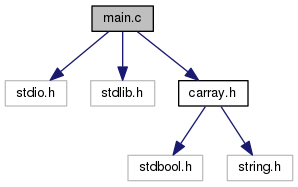
\includegraphics[width=296pt]{main_8c__incl}
\end{center}
\end{figure}
\subsection*{Macros}
\begin{DoxyCompactItemize}
\item 
\#define {\bf S\+T\+R\+I\+N\+G\+\_\+\+O\+F\+\_\+\+I\+N\+T\+\_\+\+S\+I\+ZE}~32
\end{DoxyCompactItemize}
\subsection*{Functions}
\begin{DoxyCompactItemize}
\item 
char $\ast$ {\bf chara\+\_\+of\+\_\+\+Int} ({\bf type} val)
\item 
char $\ast$ {\bf chara\+\_\+of\+\_\+\+String} ({\bf type} val)
\item 
int {\bf main\+\_\+a} (int argc, char $\ast$$\ast$argv)
\item 
int {\bf main\+\_\+b} (int argc, char $\ast$$\ast$argv)
\item 
int {\bf main} (int argc, char $\ast$$\ast$argv)
\end{DoxyCompactItemize}


\subsection{Macro Definition Documentation}
\index{main.\+c@{main.\+c}!S\+T\+R\+I\+N\+G\+\_\+\+O\+F\+\_\+\+I\+N\+T\+\_\+\+S\+I\+ZE@{S\+T\+R\+I\+N\+G\+\_\+\+O\+F\+\_\+\+I\+N\+T\+\_\+\+S\+I\+ZE}}
\index{S\+T\+R\+I\+N\+G\+\_\+\+O\+F\+\_\+\+I\+N\+T\+\_\+\+S\+I\+ZE@{S\+T\+R\+I\+N\+G\+\_\+\+O\+F\+\_\+\+I\+N\+T\+\_\+\+S\+I\+ZE}!main.\+c@{main.\+c}}
\subsubsection[{S\+T\+R\+I\+N\+G\+\_\+\+O\+F\+\_\+\+I\+N\+T\+\_\+\+S\+I\+ZE}]{\setlength{\rightskip}{0pt plus 5cm}\#define S\+T\+R\+I\+N\+G\+\_\+\+O\+F\+\_\+\+I\+N\+T\+\_\+\+S\+I\+ZE~32}\label{main_8c_a35758fd154ca32487058cd9fc6c8725e}


Definition at line 6 of file main.\+c.



\subsection{Function Documentation}
\index{main.\+c@{main.\+c}!chara\+\_\+of\+\_\+\+Int@{chara\+\_\+of\+\_\+\+Int}}
\index{chara\+\_\+of\+\_\+\+Int@{chara\+\_\+of\+\_\+\+Int}!main.\+c@{main.\+c}}
\subsubsection[{chara\+\_\+of\+\_\+\+Int(type val)}]{\setlength{\rightskip}{0pt plus 5cm}char$\ast$ chara\+\_\+of\+\_\+\+Int (
\begin{DoxyParamCaption}
\item[{{\bf type}}]{val}
\end{DoxyParamCaption}
)}\label{main_8c_aad39f2503e463ecf20a44d9eea3ded10}


Definition at line 12 of file main.\+c.

\index{main.\+c@{main.\+c}!chara\+\_\+of\+\_\+\+String@{chara\+\_\+of\+\_\+\+String}}
\index{chara\+\_\+of\+\_\+\+String@{chara\+\_\+of\+\_\+\+String}!main.\+c@{main.\+c}}
\subsubsection[{chara\+\_\+of\+\_\+\+String(type val)}]{\setlength{\rightskip}{0pt plus 5cm}char$\ast$ chara\+\_\+of\+\_\+\+String (
\begin{DoxyParamCaption}
\item[{{\bf type}}]{val}
\end{DoxyParamCaption}
)}\label{main_8c_a553c9f0d32eaceb8475fa92c26867a66}


Definition at line 19 of file main.\+c.

\index{main.\+c@{main.\+c}!main@{main}}
\index{main@{main}!main.\+c@{main.\+c}}
\subsubsection[{main(int argc, char $\ast$$\ast$argv)}]{\setlength{\rightskip}{0pt plus 5cm}int main (
\begin{DoxyParamCaption}
\item[{int}]{argc, }
\item[{char $\ast$$\ast$}]{argv}
\end{DoxyParamCaption}
)}\label{main_8c_a3c04138a5bfe5d72780bb7e82a18e627}


Definition at line 59 of file main.\+c.

\index{main.\+c@{main.\+c}!main\+\_\+a@{main\+\_\+a}}
\index{main\+\_\+a@{main\+\_\+a}!main.\+c@{main.\+c}}
\subsubsection[{main\+\_\+a(int argc, char $\ast$$\ast$argv)}]{\setlength{\rightskip}{0pt plus 5cm}int main\+\_\+a (
\begin{DoxyParamCaption}
\item[{int}]{argc, }
\item[{char $\ast$$\ast$}]{argv}
\end{DoxyParamCaption}
)}\label{main_8c_afa8958d94ce9d9f703bb182fcf516cbe}


Definition at line 26 of file main.\+c.

\index{main.\+c@{main.\+c}!main\+\_\+b@{main\+\_\+b}}
\index{main\+\_\+b@{main\+\_\+b}!main.\+c@{main.\+c}}
\subsubsection[{main\+\_\+b(int argc, char $\ast$$\ast$argv)}]{\setlength{\rightskip}{0pt plus 5cm}int main\+\_\+b (
\begin{DoxyParamCaption}
\item[{int}]{argc, }
\item[{char $\ast$$\ast$}]{argv}
\end{DoxyParamCaption}
)}\label{main_8c_a3a0604c1e565f967408274476be46c66}


Definition at line 50 of file main.\+c.


%--- End generated contents ---

% Index
\backmatter
\newpage
\phantomsection
\clearemptydoublepage
\addcontentsline{toc}{chapter}{Index}
\printindex

\end{document}
